\documentclass[runningheads]{llncs}
%
\usepackage[T1]{fontenc}
% T1 fonts will be used to generate the final print and online PDFs,
% so please use T1 fonts in your manuscript whenever possible.
% Other font encondings may result in incorrect characters.
%
\usepackage{graphicx}
\usepackage{amssymb}
\usepackage{amsmath}
%\usepackage{amsfonts}
%\usepackage{amsthm}
\usepackage{multirow}

\usepackage{tikz}

\usepackage{xspace}
\usepackage{caption}
\usepackage{subcaption}

%\usepackage[dvipsnames]{xcolor}
\definecolor{nicered}{RGB}{204,0,0}
\definecolor{lightblue}{RGB}{153,204,255}
\definecolor{nicegreen}{RGB}{0,153,0}
\usepackage{tikz}
\usetikzlibrary{decorations.pathreplacing, calligraphy}
\usetikzlibrary{decorations.pathmorphing}
\usetikzlibrary{arrows,automata}
\usetikzlibrary{arrows.meta}
\usetikzlibrary{shapes.geometric}
\usetikzlibrary{calc}
\usetikzlibrary{fpu}
\usetikzlibrary{math}

%%%%%TikZ-Styles
\tikzstyle{vertex}=[thin,circle,inner sep=0.cm, minimum size=1.7mm, fill=black, draw=black]%normal
 \tikzstyle{svertex}=[thin,circle,inner sep=0.cm, minimum size=1.3mm, fill=black, draw=black]%small
 \tikzstyle{bvertex}=[thin,circle,inner sep=0.cm, minimum size=1.7mm, fill=lightblue, draw=lightblue]%blue
 \tikzstyle{rvertex}=[thin,circle,inner sep=0.cm, minimum size=1.7mm, fill=nicered,draw=nicered]%red
 \tikzstyle{evertex}=[thin,circle,inner sep=0.cm, minimum size=1.7mm, fill=none,draw=black]%empty
 \tikzstyle{edge}=[thick, draw = gray]
 \tikzstyle{tedge}=[ultra thick, draw = black]%thick
 \tikzstyle{tredge}=[ultra thick, draw = nicered]%thick red
 \tikzstyle{tbedge}=[ultra thick, draw=lightblue]%vorher pedge
 \tikzstyle{redge}=[thick, draw = nicered]%auch rededge
 \tikzstyle{bedge}=[thick, draw = lightblue] %auch bluedge
 \tikzstyle{gedge}=[thick, draw = nicegreen] %auch grnedge
 \tikzstyle{brace} = [decorate, ultra thick, decoration = {calligraphic brace}]
 \tikzstyle{wiggly} = [decorate, decoration = snake, thick, draw = gray,]


\newcommand{\todo}[1]{\textcolor{red}{Todo:} \textcolor{blue}{#1}}
\newcommand{\todofl}[1]{\textcolor{red}{Todo for Felicia:} \textcolor{Purple}{#1}}
\newcommand{\todojo}[1]{\textcolor{red}{Todo for Jannik:} \textcolor{ForestGreen}{#1}}
\newcommand{\todojm}[1]{\textcolor{red}{Todo for Joseph:} \textcolor{orange}{#1}}


\newcommand{\NP}{\textsf{NP}}
\newcommand{\p}{\textsf{P}}
\newcommand\yes{\textsc{Yes}}
\newcommand\no{\textsc{No}}
\newcommand{\mc}{{\sc Matching Cut}}
\newcommand{\pmc}{{\sc Perfect Matching Cut}}
\newcommand{\dpm}{{\sc Disconnected Perfect Matching}}
\newcommand{\maxmc}{{\sc Maximum Matching Cut}}
\newcommand{\minmc}{{\sc Minimum Matching Cut}}
\newcommand{\mdpm}{{\sc Maximum Disconnected Perfect Matching}}
\newcommand{\dc}{{\sc $d$-Cut}}
\newcommand{\twosat}{{\sc $2$-SAT}}
\newcommand{\maxcut}{{\sc Max Cut}}
\newcommand{\etc}{{\sc Exact $3$-Cover}}
\newcommand{\eps}{{\sc Exact Positive 1-in-3 SAT}}
\newcommand{\naesat}{{\sc Not-All-Equal SAT}}
\newcommand{\maxmatch}{{\sc Maximum Matching}}
\newcommand{\mincut}{{\sc Minimum Cut}}

\newcommand{\degree}{\mathrm{degree}\xspace}
\newcommand{\dist}{\mathrm{dist}\xspace}
\newcommand{\diam}{\mathrm{diam}\xspace}

\newcommand{\tabref}[1]{{ \footnotesize (Th.~\ref{#1})}}
\newcommand{\tabcite}[1]{{ \footnotesize (\cite{#1})}}

\newtheorem{open}{Open Problem}
\newtheorem{observation}{Observation}
%\newtheorem{myclaim}{Claim}[theorem]
\spnewtheorem{myclaim}{Claim}[theorem]{\bfseries}{\itshape}
\newenvironment{claimproof}[1]{\par\noindent{\textit{Proof of the Claim.}}
\enspace#1}{\hfill \textcolor{gray}{$\vartriangleleft$}}

\newcommand{\app}{$\spadesuit$}

\newcommand\blfootnote[1]{%
    \bgroup
    \renewcommand\thefootnote{\fnsymbol{footnote}}%
    \renewcommand\thempfootnote{\fnsymbol{mpfootnote}}%
    \footnotetext[0]{#1}%
    \egroup
}

% Used for displaying a sample figure. If possible, figure files should
% be included in EPS format.
%
% If you use the hyperref package, please uncomment the following two lines
% to display URLs in blue roman font according to Springer's eBook style:
%\usepackage{color}
%\renewcommand\UrlFont{\color{blue}\rmfamily}
%\urlstyle{rm}
%
\begin{document}
%
\title{Finding Minimum Matching Cuts in $H$-free Graphs and Graphs of Bounded Radius and Diameter}
%
\titlerunning{Finding Minimum Matching Cuts}
% If the paper title is too long for the running head, you can set
% an abbreviated paper title here
%

\author{Felicia Lucke\inst{1}\orcidID{0000-0002-9860-2928} \and
Joseph Marchand\inst{2}\and
Jannik Olbrich\inst{3}\orcidID{0000-0003-3291-7342}}

%
\authorrunning{F.~Lucke, J.~Marchand and J.~Olbrich}
% First names are abbreviated in the running head.
% If there are more than two authors, 'et al.' is used.
%

\institute{Department of Computer Science, Durham University, United Kingdom \email{felicia.c.lucke@durham.ac.uk}\and
ENS Paris-Saclay, France\\ \email{joseph.marchand@ens-paris-saclay.fr} 
\and
Ulm University, Germany\\
\email{jannik.olbrich@uni-ulm.de} \blfootnote{Felicia Lucke is supported by the EPSRC
(Grant No.\ EP/X01357X/1) and Jannik Olbrich by the Deutsche Forschungsgemeinschaft (DFG) (Grant No.\ OH 53/7-1).}}




%
\maketitle              % typeset the header of the contribution
%
\begin{abstract}
A matching cut is a matching that is also an edge cut. In the problem \minmc{}, we ask for a matching cut with the minimum number of edges in the matching. We give polynomial-time algorithms for $P_7$-free, $S_{1,1,2}$-free and $(P_6 + P_4)$-free graphs, which also solve several open cases for the well-studied problem \mc{}. In addition, we show \NP-hardness for $3P_3$-free graphs, implying that \minmc{} and \mc{} differ in complexity on certain graph classes. We also give complexity dichotomies for both general and bipartite graphs of bounded radius and diameter. 

\keywords{minimum matching cut \and $H$-free graph \and diameter \and radius.}
\end{abstract}


\section{Introduction}
\label{sec:intro}
Given a graph $G$, a \emph{matching} is a set of disjoint edges. For a partition of the vertex set $V(G) = A \cup B$, the set of edges with one endvertex in $A$ and one in $B$ is an \emph{edge cut} of $G$. A \emph{matching cut} $M$ is a set of edges which is a matching and an edge cut. The number of edges $|M|$ is the \emph{size} of a matching cut.



The problem \mc, where we ask whether a given graph has a matching cut dates back to 1970 where Graham introduced it to prove a result on cube numbering, see~\cite{Gr70}. Both polynomial-time algorithms and \NP-completeness results have been published for many different graph classes such as chordal graphs~(\cite{Mo89}), graphs of bounded diameter~(\cite{BJ08}), graphs of bounded degree~(\cite{Ch84}), and graphs of large girth~(\cite{FLPR23}).
In addition, different variants and generalisations of the problem have been studied, see e.g.~\cite{BP25,GS21,LT22,RS02}.


The complexity of \mc{} on $H$-free graphs has received attention over the last years. Due to the results in~\cite{FLPR23} the only open cases are when the components of $H$ are paths or subdivided claws. This puts a special focus on $P_r$-free graphs, where $P_r$, for $r\geq 1$, is a path on $r$ vertices. In~\cite{Fe23}, Feghali showed polynomial-time solvability for $P_5$-free graphs. The first explicit result, for $P_4$-free graphs, even dates back to~\cite{Bo09}. These results were extended to $P_6$-free graphs in~\cite{LPR22}. Complementary \NP-completeness results have been published in~\cite{Fe23}, \cite{LPR22}. The currently best result shows \NP-completeness for $P_{14}$-free graphs~(\cite{LL23}). This leaves the case of $P_r$-free graphs, for $7\leq r \leq 13$, open. We contribute to closing this gap by giving in Theorem~\ref{t-p7} a polynomial-time algorithm for $P_7$-free graphs.
We further contribute to the general aim of completing the complexity dichotomy for $H$-free graphs with our polynomial-time algorithms for $S_{1,1,2}$ and $(P_6 + P_4)$-free graphs.

Only recently, in~\cite{LPR23b}, the size of a matching cut has been taken into account, when the optimisation problem \maxmc{} was introduced. Complexity dichotomies for $H$-free graphs, graphs of bounded radius and diameter, as well as for graphs of bounded degree were given. Its natural counterpart, \minmc, was introduced in~\cite{LLPR24}, where a polynomial-time algorithm for $K_{1,3}$-free graphs was given. 



It is known that for $K_{1,3}$-free graphs, \maxmc{} is \NP-hard (\cite{LPR23b}) while \mc{} and \minmc{} are polynomial-time solvable (\cite{Bo09,LLPR24}).
This raises the question whether there is a graph $H$ such that \minmc{} and \mc{} differ in complexity on $H$-free graphs. We answer this question affirmatively by showing in Theorem~\ref{t-3p3} the \NP-hardness of \minmc{} for $3P_3$-free graphs, on which \mc{} is polynomial-time solvable, see~\cite{LPR22}.


We complement this result with our proofs  
 that \minmc{} is polynomial-time solvable on $S_{1,1,2}$-free, $(P_6 + P_4)$-free, and $P_7$-free graphs. 
 We show that polynomial-time solvability on $H$-free graphs implies polynomial-time solvability on $(H+P_2)$-free graphs. Our hardness construction for $3P_3$-free graphs, together with the fact that \NP-hardness results for \mc{}, such as those for $K_{1,4}$-free~\cite{Ch84}, $H_i^*$-free graphs and graphs of high girth~\cite{LPR23a}, carry over, leave only a constant number of cases open to complete the dichotomy for $H$-free graphs.

The \emph{distance} $\dist(u,v)$ of two vertices $u$ and $v$ is the length of a shortest path between them. The \emph{eccentricity} of a vertex $v$ is the maximum distance between~$v$ and any other vertex of $G$. The \emph{radius} of $G$ is the minimum eccentricity of any vertex in $G$ and the \emph{diameter} the maximum eccentricity of any vertex in $G$.
We consider \minmc{} on graphs of bounded radius and diameter and on bipartite graphs of bounded radius and diameter. From our results, we obtain the following complexity dichotomies:


\begin{theorem}
    For an integer $r \geq 1$, \minmc{} for graphs of radius~$r$ is polynomial-time solvable if $r \leq 1$ and \NP-complete if $r \geq 2$.
\end{theorem}

\begin{theorem}
    For an integer $d \geq 1$, \minmc{} for graphs of diameter~$d$ is polynomial-time solvable if $d \leq 2$ and \NP-complete if $d \geq 3$.
\end{theorem}

\begin{theorem}
    For an integer $r \geq 1$, \minmc{} for bipartite graphs of radius~$r$ is polynomial-time solvable if $r \leq 2$ and \NP-complete if $r \geq 3$.
\end{theorem}

\begin{theorem}
    For an integer $d \geq 1$, \minmc{} for bipartite graphs of diameter~$d$ is polynomial-time solvable if $d \leq 3$ and \NP-complete if $d \geq 4$.
\end{theorem}




\section{Preliminaries}
\label{sec:prelim}
We only consider finite, simple, undirected graphs. Let $G = (V,E)$ be a graph and $v \in V$ a vertex. We denote by $n$ the number of vertices of $G$. The set $N(v) = \{u \in V| uv \in E\}$ is the \emph{neighbourhood} of $v$ and $|N(v)|$ the \emph{degree} of $v$. We say that a vertex $u\in V$ is a \emph{private neighbour} of $v$ (with respect to a set $S$) if it is only adjacent to $v$ (in $S$). Let $C\subseteq V$. We say $v$ is adjacent to $C$ if there is a vertex $u \in C$ such that $v$ is adjacent to $u$. We denote by $\dist_C(u,v)$ the length of a shortest path between $u$ and $v$ using only vertices in $C$. 

We denote by $G[C]$ the graph induced by $C$. Let $H$ be a graph. If $H$ is an induced subgraph of $G$, we write $H \subseteq_i G$ or $ G \supseteq_i H$. We say that a graph is \emph{$H$-free} if it does not contain $H$ as an induced subgraph. We denote by $sG$, $s \geq 1$, the graph arising from the disjoint union of $s$ copies of $G$.
Let $r, \ell \geq 1$ be integers. Let $P_r$, $C_r$, $K_r$ be the path, cycle, complete graph, each on $r$ vertices.
A graph is \emph{bipartite} if there is a partition $V = A \cup B$ such that all edges of $G$ have one endvertex in $A$ and one in $B$. We denote by $K_{r,\ell}$ the \emph{complete bipartite graph} with $|A| = r$ and $|B| = \ell$. We call the graph $K_{1,3} = S_{1,1,1}$ a \emph{claw}.
$S_{i,j,k}$, for $i,j,k \geq 1$, can be obtained by subdividing the edges of a claw $i,j$ and $k$ times.
Let $H^*_1$ be the ``H''-graph with vertices $u, v, x_1, x_2, y_1, y_2$ and edges $uv$, $ux_1$, $ux_2$, $vy_1$, $vy_2$. From this graph we obtain $H_i^*$ by subdividing the edge $uv$ $i-1$ times.



A \emph{red-blue colouring} of $G$ is a colouring of the vertices with red and blue, using each colour at least once. We say that a red-blue colouring is \emph{valid} if every red vertex is adjacent to at most~$1$ blue vertex and every blue vertex is adjacent to at most~$1$ red vertex.
An edge is \emph{bichromatic} if it has one red and one blue endvertex, and an edge or a vertex set $S \subseteq V$ is \emph{monochromatic} if all vertices in~$S$ have the same colour. Let $R$ be the set of red vertices of $G$. A \emph{red component} of $G$ is a connected component of the graph $G[R]$. Similarly, for $B$, the set of blue vertices, a \emph{blue component} of $G$ is a connected component of $G[B]$.
The \emph{value}~$\nu$ of a valid red-blue colouring is the number of bichromatic edges.
We make several well-known observations, see e.g.~\cite{LPR22,LPR23b}.

\begin{observation}\label{o-cutcolouring}
    A graph $G$ has a matching cut of size~$\nu$ if and only if it has a red-blue colouring of value~$\nu$. 
\end{observation}

\begin{observation}\label{o-Kr}\label{O-bipartite}
    For every $\ell \geq 3$ and $r\geq 2$, $K_\ell$ and $K_{\ell,r}$ are monochromatic in any valid red-blue colouring.
\end{observation}


\begin{observation}\label{o-degree1}
    If a graph $G$ has a vertex $v$ of degree~$1$, then the partition of the vertices into the sets $\{v\}$ and $V\setminus \{v\}$ leads to a matching cut of size~$1$.
\end{observation}




\noindent
Let $R,B \subseteq V$ with $ R \cap B = \varnothing$. A \emph{red-blue $(R,B)$-colouring} is a partial colouring of $G$ where the vertices in $R$ are coloured red and those in $B$ are coloured blue.
We say that a red-blue $(R,B)$-colouring is \emph{valid} if it can be extended to a valid red-blue colouring.
Given a pair $(R,B)$, we define propagation rules that try to extend the red-blue $(R,B)$-colouring or show that no valid red-blue $(R,B)$-colouring exists. Some of these rules have already been given in~\cite{LL19} and have been widely used since then.
Let $R' \subseteq R$ be the set of red vertices which have a blue neighbour in $B$ and similarly, let $B' \subseteq B$ be the set of blue vertices with a red neighbour in $R$. Let $Z = V\setminus (R\cup B)$.

\begin{description}
    \item[R1] Return \textsf{no}, i.e., $G$ has no valid red-blue $(R,B)$-colouring, if a vertex $v \in Z$~is:
    \begin{enumerate}
        \item adjacent to a vertex in $R'$ and a vertex in $B'$.
        \item adjacent to two vertices in $R$ and a vertex in $B'$.
        \item adjacent to two vertices in $B$ and a vertex in $R'$.
        \item adjacent to two vertices in $R$ and two vertices in $B$.
    \end{enumerate}
 

    \item[R2] Let $v\in Z$:
    \begin{enumerate}
        \item if $v$ is adjacent to two vertices in $R$ or one in $R'$, then colour $v$ red.
        \item if $v$ is adjacent to two vertices in $B$ or one in $B'$, then colour $v$ blue.
    \end{enumerate}
    \item[R3] Let $H$ be a subgraph of $G$, isomorphic to $K_{3}$, let $v \in Z \cap V(H)$.\\
        If $H$ contains a blue (resp.~red) vertex, then colour $v$ blue (resp.~red).

    \item[R4] Let $C$ be a connected component of $G[Z]$:
        \begin{enumerate}
            \item if no vertex of $C$ is adjacent to a vertex in $R$, then colour $C$ blue.
            \item if no vertex of $C$ is adjacent to a vertex in $B$, then colour $C$ red.
        \end{enumerate}

    \item[R5] Let $H$ be a subgraph of $G$, isomorphic to $K_{2,3}$, let $v \in Z \cap V(H)$.
        \begin{enumerate}
            \item If $H$ contains a blue and a red vertex, return \textsf{no}.
            \item If $H$ contains a blue (resp.~red) vertex, then colour $v$ blue (resp.~red).
            %\item If $H$ contains a red vertex then colour $v$ red.
        \end{enumerate}

\end{description}

\noindent
We say that a propagation rule is \emph{safe} if $G$ has a valid red-blue $(R,B)$-colouring before the application of the rule if and only if $G$ has a valid red-blue $(R,B)$-colouring after the application of the rule.
\begin{lemma}\label{l-propsafe}\label{l-propconnectivity}
Propagation rules R1--R5 are safe, can be applied in polynomial time, their application creates no additional red and blue components and does not increase the minimum possible value of a valid red-blue $(R,B)$-colouring.
\end{lemma}
\begin{proof}
    The safeness for R1 and R2 has already been proven in~\cite{LL19}.
    Since by Observation~\ref{o-Kr} triangles and $K_{2,3}$ are monochromatic, it follows that R3 and R5 are safe.
    To see that R4 is safe, recall that we start with at least one vertex of each colour. This guarantees the existence of vertices of both colours and, therefore, we may colour connected components adjacent to vertices of only one colour in that colour. 
    For every application of a propagation rule, we only colour vertices with the colour of one of their neighbours. Therefore, we do not create any additional coloured components.
    Note further that R1--R3 and R5 preserve the value of the colouring. R4 only decreases the maximum possible value but never results in an increase of the minimum possible value.
    \qed
\end{proof}






\noindent
The following lemmas have been shown previously for \maxmc{} in~\cite{LPR23b}.

\begin{lemma}\label{l-smalldomset}
Let $G$ be a connected graph with domination number~$g$. We can find a minimum red-blue colouring of $G$ or conclude that no such colouring exists in time $O(2^g n^{g+2})$.
\end{lemma}
\begin{proof}
Let $D$ be a dominating set of $G$ with $|D| = g$. We branch over all $2^{|D|} = 2^g$ options of
colouring the vertices of $D$ red or blue. 
For every coloured vertex without a neighbour of the other colour, we consider all $O(n)$ options to colour its neighbourhood. For every vertex $v$ with a neighbour of the other colour, we colour all its other neighbours with the colour of $v$.
Since $D$ is a dominating set, we guessed a red-blue colouring of the whole graph $G$. We can check in time $O(n^2)$ whether this colouring is a valid red-blue colouring and compute its value. If the colouring is not valid, we discard the branch, otherwise we remember its value and output the valid colouring with the smallest value. Since we consider $O(2^gn^g)$ colourings, we get a runtime of $O(2^g n^{g+2})$. \qed
\end{proof}

\begin{figure}
    \centering
    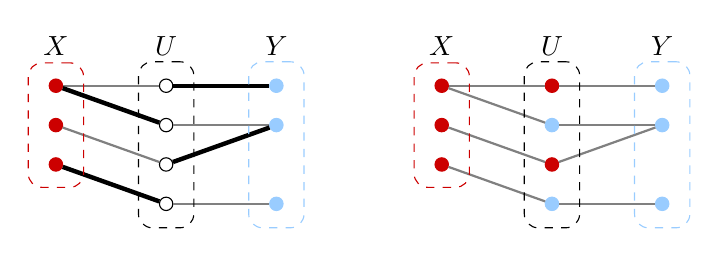
\begin{tikzpicture}
    \tikzset{
        rahmen1/.style={
            rounded corners = 5pt,
            draw,
            dashed,
            minimum width=20pt,
            minimum height=45pt
        }
    }
    \tikzset{
        rahmen2/.style={
            rounded corners = 5pt,
            draw,
            dashed,
            minimum width = 15 pt,
            minimum height = 55 pt
        }
    }
    \tikzset{
        rahmen3/.style={
            rounded corners = 5pt,
            draw,
            dashed,
            minimum width = 20pt,
            minimum height = 116pt
        }
    }
    \tikzset{
        rahmen4/.style={
            rounded corners = 5pt,
            draw,
            dashed,
            minimum width = 20pt,
            minimum height = 60pt
        }
    }
    \begin{scope}[yscale = 0.5, xscale = 0.7]
        %\node[rvertex](r1) at (-2,5){};
        %\node[rvertex](r2) at (-2,4){};
        \node[rvertex](r3) at (-2,3){};
        \node[rvertex](r4) at (-2,2){};
        \node[rvertex](r5) at (-2,1){};
        
        \node[bvertex](b1) at (2,3){};
        \node[bvertex](b2) at (2,2){};
        %\node[bvertex](b3) at (2,1){};
        \node[bvertex](b4) at (2,0){};
        
        %\node[evertex](v1) at (0,6) {};
        %\node[evertex](v2) at (0,5) {};
        %\node[evertex](v3) at (0,4) {};
        \node[evertex](v4) at (0,3) {};
        \node[evertex](v5) at (0,2) {};
        \node[evertex](v6) at (0,1) {};
        \node[evertex](v7) at (0,0) {};
        %\node[evertex](v8) at (0,-1) {};
        
        %\draw[edge] (r1) -- (v1);
        %\draw[edge] (r1) -- (v2);
        %\draw[edge] (r1) -- (v3);
        \draw[edge] (r3) -- (v4);
        \draw[tedge] (r3) -- (v5);
        \draw[edge] (r4) -- (v6);
        \draw[tedge] (r5) -- (v7);
        
        \draw[tedge] (b1) -- (v4);
        \draw[edge] (b2) -- (v5);
        \draw[tedge] (b2) -- (v6);
        \draw[edge] (b4) -- (v7);
        %\draw[edge] (b4) -- (v8);

        \node[rahmen1, nicered] (rm1) at (-2,2){};
        \node[rahmen4] (rm2) at (0,1.5){};
        %\node[rahmen3] (rm3) at (0,2.5){};
        \node[rahmen4, lightblue] (rm4) at (2,1.5){};
        \node[](x) at (-2,4){$X$};
        \node[](y) at (2,4){$Y$};
        %\node[](z) at (0,7){$Z$};
        \node[](u) at (0,4){$U$};
        \end{scope}

    \begin{scope}[yscale = 0.5, xscale = 0.7, shift = {(7,0)}]
        %\node[rvertex](r1) at (-2,5){};
        %\node[rvertex](r2) at (-2,4){};
        \node[rvertex](r3) at (-2,3){};
        \node[rvertex](r4) at (-2,2){};
        \node[rvertex](r5) at (-2,1){};
        
        \node[bvertex](b1) at (2,3){};
        \node[bvertex](b2) at (2,2){};
        %\node[bvertex](b3) at (2,1){};
        \node[bvertex](b4) at (2,0){};
        
        %\node[rvertex](v1) at (0,6) {};
        %\node[rvertex](v2) at (0,5) {};
        %\node[rvertex](v3) at (0,4) {};
        \node[rvertex](v4) at (0,3) {};
        \node[bvertex](v5) at (0,2) {};
        \node[rvertex](v6) at (0,1) {};
        \node[bvertex](v7) at (0,0) {};
        %\node[bvertex](v8) at (0,-1) {};
        
        %\draw[edge] (r1) -- (v1);
        %\draw[edge] (r1) -- (v2);
        %\draw[edge] (r1) -- (v3);
        \draw[edge] (r3) -- (v4);
        \draw[edge] (r3) -- (v5);
        \draw[edge] (r4) -- (v6);
        \draw[edge] (r5) -- (v7);
        
        \draw[edge] (b1) -- (v4);
        \draw[edge] (b2) -- (v5);
        \draw[edge] (b2) -- (v6);
        \draw[edge] (b4) -- (v7);
        %\draw[edge] (b4) -- (v8);

        \node[rahmen1, nicered] (rm1) at (-2,2){};
        \node[rahmen4] (rm2) at (0,1.5){};
        %\node[rahmen3] (rm3) at (0,2.5){};
        \node[rahmen4, lightblue] (rm4) at (2,1.5){};
        \node[](x) at (-2,4){$X$};
        \node[](y) at (2,4){$Y$};
        %\node[](z) at (0,7){$Z$};
        \node[](u) at (0,4){$U$};
        \end{scope}
    \end{tikzpicture}
    \caption{A perfect matching in $G'$ (left) and the corresponding minimum valid red-blue colouring.}\label{fig-lemma Indep Set}
\end{figure}

\begin{lemma}\label{L-Indep Set}
    Let $G = (V,E)$ be a connected graph with a red-blue $(R,B)$-colouring, for $R,B \subseteq V$. If $V\setminus (B\cup R)$ induces an independent set then it is possible in polynomial time to either find a minimum valid red-blue $(R,B)$-colouring or to conclude that $G$ has no valid red-blue $(R,B)$-colouring.
\end{lemma}


\begin{proof}
    Let $Z = V\setminus (B\cup R)$. According to R4, we colour every vertex of $Z$ that is only adjacent to vertices of one colour with this colour. Let $U$ be the set of the remaining uncoloured vertices of $Z$, i.e., the vertices with neighbours in both $R$ and $B$. Let $W = N(U)$. 
    Let $G'$ be the graph with vertex set $U\cup W$ and edge set $E(G') = \{uv | u \in U, v \in W \}$. We claim that the set of bichromatic edges of every valid red-blue $(R,B)$-colouring of $G$ is the union of a perfect matching in~$G'$ and the set of edges with one endvertex in $R$ and one in $B$.

    First suppose that $G'$ has a perfect matching $M$. Let $z\in U$. Suppose that $z$ is incident to an edge $zw\in M$. If $w\in R$ we colour $z$ in  blue. Otherwise, $w\in B$ and we colour $z$ red. Since $M$ is perfect, we coloured every vertex in $U$ and every vertex in $W$ got at most one neighbour of the other colour. We obtain a valid red-blue colouring of $G$.

    Now suppose that $G$ has a valid red-blue $(R,B)$-colouring. Every edge with an endvertex in $R$ and the other one in $B$ is bichromatic and there are no other bichromatic edges in $G[R\cup B]$. Let $M$ be the set of bichromatic edges in the remaining graph. Note that every edge of $M$ has an endvertex in $U$ so $M$ is in~$G'$. By definition of a red-blue colouring, $M$ has to be a matching. Moreover, if $z\in U$ then $z$ has a blue neighbour and a red neighbour, so it is contained in a bichromatic edge. We conclude that $M$ is perfect.
    
    Since $G'$ is bipartite we can determine a maximum matching of $G'$ in polynomial time using 
    Karp's algorithm~\cite{HK73}. Note that every perfect matching in~$G'$ has the same size. It follows that we can find a minimum valid red-blue $(R,B)$-colouring or conclude that there is no valid red-blue $(R,B)$-colouring in polynomial time. \qed
\end{proof}

\noindent
We need two results from the literature as well as more lemmas for red-blue colourings in $P_7$-free graphs.
\begin{theorem}[\cite{CS16}]\label{T-Pk}
    Let $G$ be a connected $P_k$-free graph, for $k\geq 4$. Then $G$ either has a dominating $P_{k-2}$ or a dominating $P_{k-2}$-free connected subgraph and such a subgraph can be found in polynomial time.
\end{theorem}



\begin{lemma}[\cite{LPR22}]\label{l-LPR22-monodom}
    Let $G$ be a connected graph with a red-blue $(R,B)$-colouring, for connected sets $R, B \subseteq V$. If $R$ or $B$ dominates the uncoloured vertices, it is possible to check in polynomial time if $G$ has a valid red-blue $(R,B)$-colouring.
\end{lemma}

    \begin{lemma}\label{l-prop-nonewcomp}
     Let $G$ be a graph with a red-blue $(R,B)$-colouring and let $w$ be an uncoloured vertex. We colour $w$ and propagate the colouring. If the set of uncoloured vertices is dominated by the set of coloured vertices, then we do not create an additional coloured component.
    \end{lemma}

    \begin{proof}
        Let $v$ be a coloured neighbour of $w$. If we colour $w$ the same as $v$, we clearly do not get an additional blue or red component.
        Otherwise, assume without loss of generality that we colour $w$ blue and $v$ is red and that $w$ has no blue neighbour.
        Let $Z$ be the set of uncoloured vertices and let $C$ be the connected component of $G[Z]$ containing $w$.
        By propagation of the colouring, all uncoloured neighbours of $w$ get coloured blue. If any of their coloured neighbours were blue, we did not create an additional blue component. Otherwise, all coloured neighbours of $N(w)$ are red and by propagation, $N(N(w))$ will be coloured blue.
        This propagation continues until we reach a vertex in $C$ with a blue neighbour. Note that such a vertex always exists by R4. It follows that regardless of the colour of $w$ we do not create an additional coloured component. \qed
    \end{proof}


\begin{lemma}\label{L-monodom}
Let $G = (V,E)$ be a connected $P_7$-free graph with a red-blue $(R,B)$-colouring, $R,B \subseteq V$ and $G[R]$ and $G[B]$ connected. Let $Z$ be the set of uncoloured vertices. If $Z$ is dominated by $R$ or $B$, then we can find in polynomial time a minimum red-blue colouring of $G$ or decide that no such colouring exists.
\end{lemma}

\begin{proof}
Let $B, R$ be the connected sets of blue and red vertices of $G$.
Let $Z$ be the set of uncoloured vertices. 
We may assume without loss of generality that $R$ dominates $Z$.
Hence, every connected component of $G[Z]$ is monochromatic in every valid red-blue $(R,B)$-colouring of $G$. To see this, note that a blue vertex with a red neighbour in $G[Z]$ would have a second red neighbour in $R$, a contradiction.

    Suppose that there is a vertex $x \in Z$ which is not adjacent to a vertex in $B$. Let $C$ be the connected component of $x$ in~$G[Z]$. Since $C$ was not coloured by R4, there is at least one vertex $y$ in $C$ adjacent to a vertex $b$ in $B$. If there are several such vertices, we take $y$ to be the closest to $x$ in $C$. Let $x = p_0 \, \dots \, p_k = y$ be the shortest path between $x$ and $y$ in $C$. Since $G$ is $P_7$-free, we have $k \leq 6$. Let $q_0,\dots,q_k$ be the red neighbours of $p_0,\dots,p_k$, see Figure~\ref{f-p7-dom-poly}. We branch over the $\mathcal{O}(n^6)$ colourings of $N(q_0)\cup\dots\cup N(q_k)$ and propagate the colouring. We leave $C$ uncoloured even though we already know its colour. 
    

%\begin{myclaim}\label{c-monodom-noblue}
All connected components of $G[Z]$ that contain a vertex without a blue neighbour are adjacent to $b$.
%\end{myclaim}

    \noindent\textbf{Claim~\ref{L-monodom}.1}
    \textit{
        All connected components of $G[Z]$ containing a vertex without a blue neighbour are adjacent to $b$.
        }
    %\end{myclaim}
    
    \smallskip
\begin{claimproof} 
    Let $C'$ be a connected component of $G[Z]$ containing a vertex without a blue neighbour and such that $C'$ is not adjacent to $b$. Note that this implies that $C'$ consists of at least $2$ vertices.
    Let $b' \in B$ be a blue neighbour of $C'$ which exists by R4. If $C'$ has several blue neighbours, we choose the one with the smallest distance to $b$. Let $b = b_0 \, \dots \, b_\ell=b'$, for $\ell\leq 6$ be the shortest blue path between $b$ and $b'$. 
Further, let $u \in C'$ be a neighbour of $b'$, $v \in C'$ be a neighbour of $u$ and $q_v \in R$ be the red neighbour of $v$, see Figure~\ref{f-p7-dom-poly}.     

\begin{figure}
    \centering
    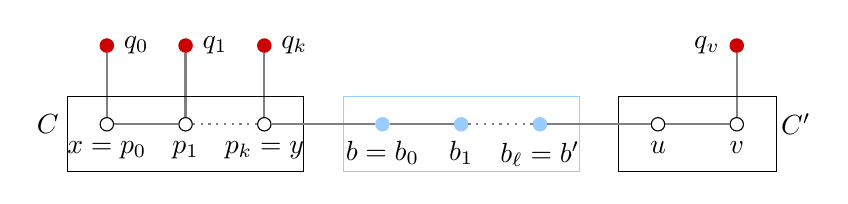
\begin{tikzpicture}
\begin{scope}
    \node[evertex, label={below:$p_k = y$}](s2p) at (2,0){};
    \node[evertex, label=below:$p_1$](s1p) at (1,0){};
    \node[evertex, label={below:$x = p_0$}](s0p) at (0,0){};

    %\node[bvertex, label = left:$b_2'$](b2p) at (-0.25, 1){};
    \node[rvertex, label = right:$q_k$](q2p) at (2,1){};
    \node[rvertex, label = right:$q_1$](q1p) at (1,1){};
    \node[rvertex, label = right:$q_0$](q0p) at (0,1){};

    \draw[edge](s0p) -- (s1p);
    \draw[edge](s0p) -- (q0p);
    \draw[edge, dotted](s1p) -- (s2p);
    \draw[edge](s1p) -- (q1p);
    \draw[edge](s2p) -- (q2p);
    %\draw[edge](s2p) -- (b2p);

    \draw[] (-0.5, -0.6) rectangle (2.5,0.35);
    \node[] (c) at (-0.75,0){$C$};
    
\end{scope}


\begin{scope}[shift = {(3.5,0)}]
    \node[bvertex, label = {below:$b = b_0$}](t0) at (0,0){};
    \node[bvertex, label = below:$b_1$](t1) at (1,0){};
    %\node[bvertex, label = below:$t_{k}$](tk1) at (2,0){};
    \node[bvertex, label = {below:$b_\ell = b' $}](tk) at (2,0){};

    \draw[edge](t0) -- (t1);
    \draw[edge, dotted](t1) -- (tk);
    %\draw[edge](tk1) -- (tk);

    \draw[lightblue] (-0.5,-0.6) rectangle (2.5,0.35);
    %\node[] (bw) at (1.5, 0.6){$B_w$};

    
    
\end{scope}


\begin{scope}[shift = {(8,0)},  xscale = -1]
    \node[evertex, label=below:$v$](s2) at (0,0){};
    \node[evertex, label=below:$u$](s1) at (1,0){};

    %\node[bvertex, label = right:$b_2$](b2) at (-0.25, 1){};
    \node[rvertex, label = left:$q_v$](q2) at (0,1){};
    %\node[rvertex, label = left:$q_1$](q1) at (1,1){};

    \draw[edge](s1) -- (s2);
    %\draw[edge](s1) -- (q1);
    \draw[edge](s2) -- (q2);
    %\draw[edge](s2) -- (b2);

    \draw[] (-0.5, -0.6) rectangle (1.5,0.35);
    \node[] (c) at (-0.75,0){$C'$};
    
\end{scope}

    \draw[edge](s2p) -- (t0);
    \draw[edge](s1) -- (tk);

\end{tikzpicture}
    \caption{The connected components $C$ and $C'$ of $G[Z]$.}
    \label{f-p7-dom-poly}
\end{figure}

    We claim that $p_0 \, \dots \, p_k \, b_0 \, \dots \, b_\ell\, u\, v \, q_v$ is an induced path of length at least~$7$. Note first that, by assumption, $x$ is not adjacent to any of $b_0,\dots,b_\ell$. 
   Further, the choice of $y$ implies that none of $p_1, \dots, p_{k-1}$ was adjacent to any of $b_0,\dots,b_\ell$.
   Any uncoloured neighbour of $y$ is in $C$ and remains uncoloured. Therefore, and since $y$ did not have two blue neighbours before colouring the neighbourhood of $q_0, \dots, q_k$, $y$ has no neighbour in $b_1, \dots, b_\ell$.
    Note further that no vertex of $C$ can be adjacent to a vertex in $C'$.
   If $q_v$ is a neighbour of one of $p_0, \dots , p_k$ and was uncoloured before colouring the neighbours of $q_0, \dots, q_k$, it would belong to $C$ and thus, remains uncoloured. Also, if $q_v$ would be one of the red neighbours of $p_0, \dots , p_k$ that is, $q_v$ is one of $q_0, \dots, q_k$, $v$ would have been coloured. For the same reason, $q_v$ cannot be adjacent to any of the $b_0, \dots, b_\ell$ or to $u$.
Therefore, $p_0 \, \dots \, p_k \, b_0 \, \dots \, b_\ell\, u\, v \, q_v$ is indeed an induced $P_7$, a contradiction to our assumption that $G$ is $P_7$-free.
\end{claimproof}


    By Claim~\ref{L-monodom}.1, we may assume that if there is any uncoloured vertex without a blue neighbour, then there is a vertex $b$ in $B$ which is adjacent to all connected components containing such a vertex.
    Since the connected components of $G[Z]$ are monochromatic, we branch over the $O(n)$ colourings of the components adjacent to $b$ and propagate the colouring using R1--R5. If we obtain a no-answer, we discard the branch.


    Therefore, we may assume that every vertex in $Z$ is adjacent to a blue and a red vertex. This implies that in every valid red-blue $(R,B)$-colouring of $G$, every vertex in $Z$ contributes~$1$ to the value of the colouring. Therefore, the value of all valid red-blue $(R,B)$-colourings is the same, and we apply Lemma~\ref{l-LPR22-monodom}. We either find a valid red-blue colouring or conclude that no such colouring exists. In the first case we remember its value, in the latter, we discard the branch.





Whenever we discard a branch, we consider the next. 
We remember the value of every valid red-blue colouring which we obtain and return the minimum of their values or that no such colouring exists.
The correctness of our algorithm follows from its description.
We consider in total $O(n^7)$ branches, each of which can be processed in polynomial time. Therefore, our algorithm runs in polynomial time.
\qed
\end{proof}

\begin{lemma}\label{l-ddmp}
    Let $G$ be a connected $P_7$-free graph with a connected dominating set~$D$. Let $D'$ be a dominating set of $G[D]$ of size $g$. We can find in polynomial time a minimum red-blue colouring of $G$ in which $D'$ is monochromatic or conclude that no such colouring exists.
\end{lemma}
\begin{proof}
    Let $D$ be a dominating set of $G$ and $D'$ a dominating set of $G[D]$ of size~$g$.
    Without loss of generality, we colour $D'$ red.
    We branch over all $\mathcal{O}(n^g)$ colourings of the neighbourhood of $D'$. Note that this implies that $D$ is coloured.
    We propagate the colouring exhaustively using R1--R5. If we obtain a no-answer we discard the branch, otherwise we continue.
    Let $R$ be the set of red vertices and $B$ the set of blue vertices.

    Since $D$ is dominating and coloured, every uncoloured vertex has a neighbour in $D$.
    Note that every blue vertex in $D$ has a red neighbour in $D'$. Thus, the neighbours of the blue vertices in $D$ are coloured blue by propagation. Therefore, every uncoloured vertex has exactly one red neighbour in $D$ resulting in a monochromatic dominating set. 
    We apply Lemma~\ref{L-monodom} to either find a minimum red-blue $(R,B)$-colouring whose value we remember or conclude that no such colouring exists and discard the branch. 

    Whenever we discard a branch, we consider the next. If no branch returns a valid red-blue colouring we return that no such colouring exists, otherwise we return the obtained red-blue colouring with the minimum value.

    The correctness of our algorithm follows from its description. Every branch can be processed in polynomial time, and we consider $O(n^g)$ branches. Therefore, our algorithm runs in polynomial time.
    \qed
\end{proof}

    
\section{Polynomial-Time Results}
\label{sec:poly}

\noindent
Before showing our main results in this section, we first state several results where the proof methods of \maxmc{} directly carry over to \minmc. To obtain the following results we reuse the proofs from~\cite{LPR23b} and~\cite{Lu25}, apply Lemma~\ref{l-smalldomset} and~\ref{L-Indep Set} instead of the corresponding results for \maxmc{}, and replace \emph{maximum} by \emph{minimum}.


\begin{theorem}\label{T-P6}
    \minmc{} is solvable in polynomial time for $P_6$-free graphs.
\end{theorem}

\begin{theorem}\label{T-H+P2}
    Let $H$ be a graph. If \minmc{} is polynomial-time solvable for $H$-free graphs, then it is so for $(H+P_2)$-free graphs.
\end{theorem}

\begin{theorem}\label{t-diam2}
    \minmc{} is solvable in polynomial time for graphs of diameter at most $2$.
\end{theorem}


\begin{theorem}
    \minmc{} is solvable in polynomial time for bipartite graphs of radius at most~$2$.
\end{theorem}

\begin{theorem}
    \minmc{} is solvable in polynomial time for bipartite graphs of diameter at most~$3$.
\end{theorem}

\noindent
We now get to our main results of this section. All three results solve open cases for \mc.

\begin{theorem}\label{t-s112}
    \minmc{} is solvable in polynomial time for $S_{1,1,2}$-free graphs.
\end{theorem}

\begin{proof}
    Let $G$ be a $S_{1,1,2}$-free graph.
    We first check whether $G$ has a vertex of degree~$1$ leading to a minimum matching cut, see Observation~\ref{o-degree1}. 
    Therefore, we may assume that $G$ has minimum degree $2$. 
    We apply Observation~\ref{o-cutcolouring} and search for a minimum red-blue colouring of $G$.

    We branch over all $O(n^2)$ options of choosing two adjacent vertices $x$ and $y$ of $G$. For every such pair we colour $x$ red and $y$ blue. We propagate the red-blue $(\{x\}, \{y\})$-colouring exhaustively which takes polynomial time by Lemma~\ref{l-propsafe}. If we get a no-answer, we discard the branch, otherwise, we obtained a red set $R$ and a blue set $B$.
    Let $Z$ be the set of uncoloured vertices.

    \begin{myclaim}\label{C-clawfree}
        $G[Z]$ is claw-free.
    \end{myclaim}
    
    \smallskip
    \begin{claimproof}
    Suppose for a contradiction that there is a claw $C$ in $G[Z]$, consisting of vertices $u, v_1, v_2, v_3$ such that $u$ is adjacent to $v_1, v_2, v_3$.

    Consider a shortest path from $C$ to $x$ avoiding blue vertices. Note that such a path always exists, otherwise $C$ would be blue by R4. Suppose that there is a path starting from $u$. Let $u = p_0 \, p_1 \, \dots \, p_k = x$ be such a path and set $p_{k+1} = y$. Since all neighbours of $y$ except $x$ are blue, the path $p_0 \, \dots \, p_{k+1}$ is induced. If $u$ was adjacent to $x$ it would be coloured by R2. Since it is uncoloured we have $k \geq 1$. Note that $p_2$ is not adjacent to any vertex in $C$, otherwise there is a shorter path from $C$ to $x$. If at least two of $v_1, v_2, v_3$, say $v_1$ and $v_3$, are not adjacent to $p_1$, then $u, v_1, v_3, p_1, p_2$ induce $S_{1,1,2}$. Hence, we may assume $v_1$ and $v_3$ are adjacent to $p_1$. If $p_3 \neq y$, an edge from $p_3$ to $C$ would imply the existence of a shorter path. Recall that $y$ is not adjacent to $C$. Thus, in any case, $p_3$ cannot be adjacent to $v_1$ or $v_3$ and $p_1, v_1, v_3, p_2, p_3$ induce $S_{1,1,2}$, a contradiction.  

    It remains to consider the case where no shortest path from $C$ to $x$ avoiding blue vertices starts from $u$. We may assume without loss of generality that there is such a path starting from $v_1$. Let $v_1 = p_0 \, \dots \, p_k = x$ be such a path. Note that from the fact that $v_1$ is uncoloured, we get $k \geq 1$. If $p_1$ is neither adjacent to $v_2$ nor to $v_3$ then $u,v_1,p_1,v_2,v_3$ is an induced $S_{1,1,2}$. As before, neither $p_2$ nor $p_3$ can be adjacent to $v_1$ or $v_3$. Hence, we find an $S_{1,1,2}$ with $p_1, v_1, v_3, p_2, p_3$.
    \end{claimproof}



\smallskip
\noindent   
    Suppose first that $G[Z]$ is a cycle with at least $4$ vertices. Every vertex in $G[Z]$ has at most one red and one blue neighbour which is neither $x$ nor $y$. Two neighbours on the cycle do not have a common coloured neighbour, since otherwise they would have been coloured. Thus, we can find an induced $S_{1,1,2}$ by taking a vertex, its two neighbours on the cycle, one of its coloured neighbours, say $v$ and a neighbour of $v$ on the shortest coloured path towards $x$ and $y$.


    Let now $Z_\Delta$ be the set of edges of $G[Z]$ which are contained in some triangle. 
    Let $C_1, \dots, C_r$ be the connected components of $G[Z_\Delta]$.
    Then, each of $C_1, \dots, C_r$ is monochromatic.
    We apply propagation rule R2 on each of the sets $C_1, \dots, C_r$ to eventually extend them with other vertices which will necessarily get the same colour. If due to the propagation two sets $C_1, \dots, C_r$ share a vertex, we unite them and continue the propagation with this set.
    This propagation might change the number of sets. After the propagation, we update the integer $r$ and assume that we have $r$ sets $C_1, \dots, C_r$.
    
    Let $Z'\subseteq Z$ be the set of edges not contained in $Z_\Delta$.
    Since $G[Z]$ is claw-free and not a cycle, the graph induced by the edges of $Z'$ is a collection of paths.
       
    

    We contract each of the sets $X,Y, C_1, \dots, C_r$ to a single vertex and obtain a graph $G'$. Note that this might result in a multigraph. 
    
    \begin{myclaim}
        $G$ has a red-blue $(x,y)$-colouring of value~$\mu$ if and only if $G'$ has an $(x,y)$-cut of size~$\mu$.
    \end{myclaim}
    \begin{claimproof}
        Suppose $G$ has a red-blue $(x,y)$-colouring of value~$\mu$. Then, every component $X,Y, C_1, \dots, C_r$ is monochromatic, that is, no bichromatic edge is inside one of these components. Thus, every bichromatic edge in $G$ corresponds to an edge in $G'$, and the cut of $G$ induced by the bichromatic edges is a cut in~$G'$ of the same size.

        For the other direction suppose that $G'$ has an $(x,y)$-cut of size~$\mu$. This cut partitions the vertex set into two sets. We colour the set containing $x$ red and the set containing $y$ blue. Recall that the graph induced by the vertex set of $Z'$ is a collection of disjoint paths. Thus, every vertex in $G$ is adjacent to at most one vertex of the other colour and the colouring is valid. Note that the value of the colouring equals the size of the cut in $G'$.
    \end{claimproof}
    

    We follow this approach for every pair of vertices $x,y$. Whenever we get a contradiction, we discard the branch. For every branch that leads to a valid red-blue colouring, we remember the value of this colouring and minimize over all values of all valid red-blue colourings obtained in the process.

    The correctness of our algorithm follows from its description. Regarding the running time, note that by Lemma~\ref{l-propsafe} the propagation of the colouring can be done in polynomial time. Further, we consider $O(n^2)$ branches and for each branch, we apply a minimum cut algorithm. This can be done, for example, in $O(n^2|E(G)|)$, using Dinic's algorithm, see~\cite{Di70}.
    Thus, our algorithm runs in polynomial time.
 \qed
\end{proof}

\noindent
For the proof of Theorem~\ref{T-P6+P4free}, we need the following lemma and apply Theorem~\ref{T-P6}.


\begin{lemma}\label{L-P4free}
    Let $G$ be a connected $P_4$-free graph on $n$ vertices. Then, $G$ has at most $2n$ different valid red-blue colourings.
\end{lemma}
\begin{proof}

    It is well-known (see e.g.\ Lemma $2$ in~\cite{KP20}) that every connected $P_4$-free graphs has a spanning complete bipartite subgraph $K_{k,l}$ for some integers $1 \leq k \leq l$. 
    By Observation~\ref{O-bipartite}, we get that $K_{k,l}$ is monochromatic if $k\geq 2$ and $l\geq 3$. If $k = 1$, that is, $G$ has a spanning star, there are at most $2n$ options to colour the graph ($2$ options to colour the centre vertex and $n$ options to choose at most one vertex with a colour different from that of the centre vertex).
    Otherwise, we get that $k = 2$ and $l=2$, that is, $G$ has a spanning $C_4$. It is easy to verify that there are at most $6 \leq 2n$ valid options to colour a $C_4$.
    Therefore, $G$ has at most~$2n$ different valid red-blue colourings. \qed
\end{proof}

\begin{theorem}\label{T-P6+P4free}
\textsc{Minimum Matching Cut} is polynomial-time solvable for $(P_6+P_4)$-free graphs.
\end{theorem}

\begin{proof}
Let $G$ be a $(P_6+P_4)$-free graph. If $G$ is $P_6$-free, we can determine whether $G$ has a minimum matching cut using Theorem~\ref{T-P6}. Thus, we may assume that $G$ is not $P_6$-free. Let $P$ be an induced $P_6$ of $G$. Note that we can find $P$ in $O(n^6)$.
We apply Observation~\ref{o-cutcolouring} and search for a minimum red-blue colouring of $G$.

We branch over all possible colourings of $P$ and $N(P)$. There are at most $O(n^{6})$ such colourings since there is a constant number of colourings of $P$ and every vertex of $P$ has at most one neighbour of the opposite colour. If the colouring of $P$ and $N(P)$ is monochromatic, say all vertices are blue, then we branch over all $O(n)$ options of colouring one of the uncoloured vertices red. 
Let $B$ be the set of blue vertices of $G$ and let $R$ be the set of red vertices of $G$. We propagate the $(R,B)$-colouring using rules R1--R5. If we get a contradiction, we discard the branch.

    Since each of the six vertices of $P$ has at most one neighbour of the opposite colour, there are at most $6$ red and $6$ blue components in $G$.
    By Lemma~\ref{l-propconnectivity} this still holds after the propagation. 
Let $Z$ be the set of uncoloured vertices of $G$. Note that $G[Z]$ is $P_4$-free.
We make a first observation.
 


    \smallskip
        \begin{myclaim}\label{C-CleanC}
         Let $v$ be a coloured vertex, say $v$ is blue. Suppose $v$ is adjacent to $w \in Z$. We colour $w$ and propagate the colouring. Regardless of the colour of $w$, we did not create an additional blue or red component.
        \end{myclaim}
        \begin{claimproof} 
            If $w$ is coloured blue, then, since $w$ is adjacent to the blue vertex $v$, we did not create a new connected component.
            
            Now assume that $w$ is coloured red. Let $C$ be the connected component of~$G[Z]$ containing $w$. Then, since $v$ is blue, we colour all uncoloured neighbours of~$w$ red. 
            Note that by R4, the component $C$ has at least one vertex adjacent to a vertex in a red component.
            Let $p$ be such a vertex.
            Note that since $C$ is $P_4$-free, we have $\diam(C)\leq 2$.
            Therefore, either $w$ is adjacent to $p$ or they have a common neighbour.
            Since all neighbours of $w$ in~$C$ are coloured red, $p$ has two red neighbours and is therefore coloured red as well.
           Thus, $w$ is connected by a red path to a red component of $G$ and we did not create a new coloured component.
        \end{claimproof}

   \paragraph*{Blue Coast Processing}
    We repeat the following steps until we hit in Step~2 the same blue component a second time. Note that this requires at most $7$ iterations, since $G$ has at most $6$ blue components. 
    In the case where no connected component of size at least~$2$ remains in $G[Z]$, we apply Lemma~\ref{L-Indep Set} and either discard the branch or found a valid red-blue colouring.
    \begin{enumerate}
        \item Pick a connected component of $G[Z]$ of size at least~$2$.
        \item Pick a blue neighbour $w$ of this component.
        \item Let $s_1,s_2 \in C$ such that $s_1 w, s_1s_2 \in E(G)$. Let $q_1$ (resp.~$q_2$) be the only red neighbour of $s_1$ (resp.~$s_2$) and $b_2$ the only blue neighbour of $s_2$, if they exist. 
        \item Branch over all $O(n^5)$ colourings of $C\cup N(w)\cup N(q_1)\cup N(q_2)\cup N(b_2)$.
    \end{enumerate}

    \noindent
    Let $C$ be the currently chosen connected component of $G[Z]$. Note  that by~R4, every connected component of $G[Z]$ has a blue neighbour. Let $w$ be a blue neighbour of $C$ in the blue component $B_w$. Suppose first that we have not chosen $B_w$ before.
    Then $s_1$ and $s_2$ can each have at most one neighbour of the same colour, otherwise they would have been coloured by R2. Further, $C$ is $P_4$-free and has, by Lemma~\ref{L-P4free}, at most $O(n)$ red-blue colourings.
    

    
    Suppose now that we picked the blue component $B_w$ before, using a vertex~$v$. That is, there was a connected component $C'$ of $G[Z]$ with a blue neighbour~$v$ in~$B_w$. Let $s_1', s_2', q_1', q_2'$ and $b_2'$ be the vertices and neighbours of $C'$ considered while processing $C'$.
    Note that if there are several vertices $w \in B_w$ which are adjacent to $C$, we may assume that $\dist_B(v,w)$ is minimized among the options for~$w$.
    Further, $v \neq w$, since the neighbours of $v$ were coloured when processing $C'$ and $w$ has an uncoloured neighbour.
    Let now $s_1,s_2 \in C$ such that $s_1$ is adjacent to both $w$ and $s_2$. Let $v \, t_1 \, \ldots \, t_k \, w$ with $t_1,\ldots,t_k \in B_w$ be a shortest blue path between $v$ and $w$. Note that this implies that the path is an induced~$P_{k+2}$.

    \begin{figure}
        \centering
        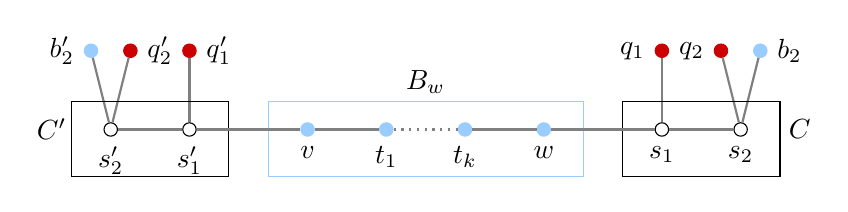
\begin{tikzpicture}
\begin{scope}
    \node[evertex, label=below:$s_2'$](s2p) at (0,0){};
    \node[evertex, label=below:$s_1'$](s1p) at (1,0){};

    \node[bvertex, label = left:$b_2'$](b2p) at (-0.25, 1){};
    \node[rvertex, label = right:$q_2'$](q2p) at (0.25,1){};
    \node[rvertex, label = right:$q_1'$](q1p) at (1,1){};

    \draw[edge](s1p) -- (s2p);
    \draw[edge](s1p) -- (q1p);
    \draw[edge](s2p) -- (q2p);
    \draw[edge](s2p) -- (b2p);

    \draw[] (-0.5, -0.6) rectangle (1.5,0.35);
    \node[] (c) at (-0.75,0){$C'$};
    
\end{scope}


\begin{scope}[shift = {(2.5,0)}]
    \node[bvertex, label = {below:$v$}](t0) at (0,0){};
    \node[bvertex, label = below:$t_1$](t1) at (1,0){};
    \node[bvertex, label = below:$t_{k}$](tk1) at (2,0){};
    \node[bvertex, label = {below:$w $}](tk) at (3,0){};

    \draw[edge](t0) -- (t1);
    \draw[edge, dotted](t1) -- (tk1);
    \draw[edge](tk1) -- (tk);

    \draw[lightblue] (-0.5,-0.6) rectangle (3.5,0.35);
    \node[] (bw) at (1.5, 0.6){$B_w$};

    
    
\end{scope}


\begin{scope}[shift = {(8,0)},  xscale = -1]
    \node[evertex, label=below:$s_2$](s2) at (0,0){};
    \node[evertex, label=below:$s_1$](s1) at (1,0){};

    \node[bvertex, label = right:$b_2$](b2) at (-0.25, 1){};
    \node[rvertex, label = left:$q_2$](q2) at (0.25,1){};
    \node[rvertex, label = left:$q_1$](q1) at (1,1){};

    \draw[edge](s1) -- (s2);
    \draw[edge](s1) -- (q1);
    \draw[edge](s2) -- (q2);
    \draw[edge](s2) -- (b2);

    \draw[] (-0.5, -0.6) rectangle (1.5,0.35);
    \node[] (c) at (-0.75,0){$C$};
    
\end{scope}

    \draw[edge](s1p) -- (t0);
    \draw[edge](s1) -- (tk);

\end{tikzpicture}
        \caption{The connected components $C$ and $C'$ adjacent to $B_w$ as considered in Claim~\ref{c-p6p4-indP6}.}
        \label{f-p4p6}
    \end{figure}



    \smallskip
     \begin{myclaim}\label{c-p6p4-indP6}
     There is an induced $P_6$ in $G[s_1, s_2, s_1', s_2', v, t_1, \dots, t_k, w]$. We may colour this path and its neighbourhood in polynomial time.
    \end{myclaim}
    \begin{claimproof}
        Note first that, due to R3, $s_2'$ is not adjacent to $v$ and~$s_2$ is not adjacent to $w$.
        Additionally, $s_i'$ and $s_j$, with $i,j\in \{1,2\}$, are not adjacent, otherwise $s_j$ would have been in $C'$.
        Further, $s_j$ cannot be adjacent to~$v$, since the neighbours of $v$ have been coloured while processing $C'$.
        If $w$ was uncoloured before processing $C'$, it cannot be adjacent to $s_i'$, otherwise $s_j$ would have been in $C$. If $w$ was blue before processing $C'$, then since $v \neq w$ and $s_1'$ had at most one blue neighbour, $w$ is not adjacent to $s_1'$. Also, $w$ is not adjacent to $s_2'$ since otherwise $w = b_2'$ and therefore, $s_1$ was coloured.
        Thus, we know that $G[v,s_1', s_2', w, s_1, s_2]$ is an induced $2P_3$. However, there might be edges from $t_\ell, \ell  \in \{1,\dots, k\}$ to $s_1', s_2', s_1$, and~$s_2$. 

        If there was an edge $t_\ell s_1$ or $t_\ell s_2$, for $\ell \in \{1,\dots, k\}$, then we would have chosen $t_\ell$ instead of $w$ due to the shorter distance from $v$ to $t_\ell$.
        Thus, there might only be edges from $t_\ell, \ell  \in \{1,\dots, k\}$ to $s_1', s_2'$.
        If there is no such edge, then $s_2'\, s_1'\, v\, t_1\, \dots\, t_{k}\, w\, s_1\, s_2$ is an induced path of length at least $6$ and we branch over all $O(n^5)$ colourings of $C\cup N(w)\cup N(q_1)\cup N(q_2)\cup N(b_2)$.
        Otherwise, let $\ell \in \{1,\dots, k\}$ be the largest integer such that one of $s_1'$ and $s_2'$ is adjacent to $t_\ell$.
        
        If exactly $s_1'$ is adjacent to $t_\ell$, then $P' = s_2'\,s_1'\, t_\ell\, \dots\, t_{k}\, w\, s_1\, s_2$ is an induced path. If exactly $s_2'$ is adjacent to $t_\ell$, then $P' = s_1'\,s_2'\, t_\ell\, \dots\, t_{k}\, w\, s_1\, s_2$ is an induced path. In both cases, $P'$ contains an induced $P_6$.
        Note that $P'$ has length at most~$10$, since a $P_{11}$ contains an induced $P_6+P_4$. Thus, $k-\ell+1\leq 5$.
        We branch over all $O(n^{10})$ colourings of $C \cup N(t_\ell) \cup \dots \cup N(t_{k}) \cup N(w) \cup N(q_1) \cup N(q_2) \cup N(b_2).$

        Otherwise, both $s_1'$ and $s_2'$ are adjacent to $t_\ell$. Since $s_1', s_2', t_\ell$ form a triangle, by R3, they have all been coloured while processing $C'$.
        Note that $t_\ell$ is adjacent to $w$ since otherwise there is an induced $P_6$ contained in the induced path $s_1'\,t_\ell\,t_{\ell+1}\, \dots \, w\, s_1 \, s_2$.
        Therefore, $w$ was already blue when $C'$ was processed since otherwise $w$, $s_1$ and $s_2$ were in $C'$ and got coloured.
        It follows that $t_\ell$ is not adjacent to $v$; otherwise, it would have been adjacent to two blue vertices before processing $v$. Let $P' = v\,t_{1}\,\ldots\,t_{k}\,w\,s_1\,s_2$. Then, $P'$ contains an induced $P_6$. We branch over all $O(n^{11})$ colourings of \[C\cup N(w)\cup N(t_1)\cup \ldots\cup N(t_{k})\cup N(q_1)\cup N(q_2)\cup N(b_2). \]
    \end{claimproof}


   
       

        \smallskip\noindent
        Let $P'$ be the induced $P_6$ constructed in Claim~\ref{c-p6p4-indP6}. We may assume that $P'$ and its neighbourhood are coloured. We apply the propagation rules R1--R5 again. If we get a no-answer, we discard the branch, otherwise we continue.

        \begin{myclaim}\label{C-StrongP}
         No uncoloured vertex and no red vertex of $G$ adjacent to an uncoloured vertex is adjacent to $P'$.
        \end{myclaim}
        \begin{claimproof}
            Note that we coloured all neighbours of $P'$. Thus, $P'$ has no uncoloured neighbours. Let $q$ be a red vertex adjacent to $P'$. Suppose for a contradiction that $q$ has an uncoloured neighbour $x$. Then, $q$ is not adjacent to a blue vertex of $P'$, otherwise $x$ would have been coloured. Suppose that $q$ is adjacent to $s_i$, for $i \in \{1,2\}$; the case of $s'_i$ works the same way. If $q$ was uncoloured when $s_i$ got coloured, then both $q$ and $x$ were in $C$ and therefore got coloured together with $s_i$. Otherwise, $q$ was $q_i$, the only red neighbour of $s_i$ and $x$ would have been coloured.
        \end{claimproof}
        
    
     \paragraph*{Red Coast Processing}

    Recall that $Z$ is the set of uncoloured vertices. If $G[Z]$ only consists of isolated vertices, we apply Lemma~\ref{L-Indep Set}. We either obtain a valid red-blue colouring in which case we remember its value or no such colouring exists and we discard the branch.

    So in the following, we may assume that $G[Z]$ has some connected component of size at least~$2$. After proving in Claim~\ref{C-Private} that every red vertex has neighbours in at most one uncoloured component, we show that their structure is very restricted.

    
        \begin{myclaim}\label{C-Private}
         Let $K$ be a connected component of $G[Z]$ of size at least $2$. Let $q\in R$ be a red neighbour of $K$. Every uncoloured neighbour of $q$ is in $K$.
        \end{myclaim}
        \begin{claimproof}
        Recall that by R4, every uncoloured component has a red neighbour.
            Suppose for a contradiction that there is a vertex $u\in Z$ which is adjacent to $q$ but not contained in $K$.
            Let $x_1,x_2 \in V(K)$ such that $q\,x_1, x_1\, x_2 \in E(G)$. Then, $q\,x_2\notin E(G)$, since otherwise $x_1$ and $x_2$ would be coloured by R3. Hence, $P'' = x_2\,x_1\,q\,u$ is an induced $P_4$. By Claim~\ref{C-StrongP}, $P' + P''$ is an induced $P_6+P_4$, a contradiction.
        \end{claimproof}

        \smallskip\noindent
        Let $K$ be a connected component of $G[Z]$ of size at least $2$.

        \smallskip\noindent
        \textbf{Case 1:} Suppose that there is a red vertex $q$ with at least two neighbours in $K$, say $x_1$ and $x_2$. Then $x_1$ and $x_2$ cannot be adjacent since otherwise they would be coloured by R3. Since $x_1$ and $x_2$ are in the same connected component $K$ of $G[Z]$, they are connected by a path in $K$. If the shortest path in $K$ between them has length at least three, it is an induced $P_4$, say $P''$, and by Claim~\ref{C-StrongP} we obtain that $P' + P''$ is an induced $P_6+P_4$. Thus, the distance of $x_1$ and $x_2$ is exactly two and therefore there is a vertex $x_3 \in K$ such that $x_3$ is adjacent to both $x_1$ and $x_2$. Note that if $q$ was adjacent to $x_3$ then $x_1,x_2$ and $x_3$ would be red by R3.

        
        \begin{myclaim}\label{C-K}
            $K = \{x_1,x_2,x_3\}$
        \end{myclaim}
        \begin{claimproof}
            Suppose for a contradiction that there is an additional vertex $x_4$ in $K$. Without loss of generality, we may assume that $x_4$ is adjacent to $x_1$ or $x_3$. 
            Suppose first that $x_4$ is adjacent to $x_1$. Then, $x_4$ has to be adjacent to at least one of $q$ and $x_2$, since, by Claim~\ref{C-StrongP}, $x_2\,q\,x_1\,x_4$ cannot be an induced $P_4$. Adjacency to $q$ leads to a triangle $x_4\,q\,x_1$, implying that $x_1$ and $x_4$ are coloured by R3, a contradiction. Therefore, $x_4$ is adjacent to $x_2$. This implies that $K_{2,3}$ is a spanning subgraph of $K\cup \{q\}$. Thus, $K$ has to be monochromatic and coloured red by R5, a contradiction.
            
            Consider now the case where $x_4$ is not adjacent to $x_1$. Hence, $x_4$ is adjacent to~$x_3$. Then, $x_4$ is adjacent to $q$ or to both $x_1$ and $x_2$, since, by Claim~\ref{C-StrongP}, neither $q\,x_1\,x_3\,x_4$ nor $q\,x_2\,x_3\,x_4$ are induced $P_4$s. Note that by assumption $x_4$ is not adjacent to $x_1$. 
            If $x_4$ is adjacent to $q$, then $K\cup \{q\}$ has again $K_{2,3}$ as a spanning subgraph and by R5, we get a contradiction. Thus, in all cases, we get a contradiction, and the claim holds. 
        \end{claimproof}

        \smallskip\noindent
        From Claim~\ref{C-K} we got that $K = \{x_1, x_2, x_3 \}$. In the following, we analyse the blue neighbours of $K$. Let $y_i$ be the blue neighbour (if it exists) of $x_i$ for $i\in \{ 1,2,3\}$. Note that $y_1, y_2$ and $y_3$ are not necessarily different.
        Depending on the blue neighbours, we colour such a component $K$ as follows:
        \begin{enumerate}
            \item  If $x_1$ and $x_2$ both have a blue neighbour, colour $K$ red.
            \item If exactly $x_1$ and $x_3$ have a blue neighbour, colour $x_2$ red and $x_1, x_3$ blue.
            \item If exactly $x_2$ and $x_3$ have a blue neighbour, colour $x_1$ red and $x_2, x_3$ blue.
            \item If exactly $x_1$ has a blue neighbour, colour $x_2$ red.
            \item If exactly $x_2$ has a blue neighbour, colour $x_1$ red.
            \item If exactly $x_3$ has a blue neighbour, colour $x_1$ red.
        \end{enumerate}


        \begin{myclaim}
         $G$ has a minimum red-blue $(R,B)$-colouring before applying the aforementioned colouring rules if and only if it has one afterwards.
        \end{myclaim}
        \begin{claimproof}
            \textit{1.} If $x_3$ is coloured blue, then so are $x_1$ and $x_2$. Thus, $q$ has two blue neighbours, a contradiction. Hence, we can safely colour $x_3$ red. Then $x_1$ and $x_2$ have to be coloured red, too.\\
            \textit{2.-3.} If exactly $y_1$ (or $y_2$ by symmetry) and $y_3$ exist then there are $2$ ways of colouring $K$. Either we colour $K$ red or we only colour $x_2$ red and $x_1$ and $x_3$ blue. Both colourings contribute $2$ to the value of the red-blue colouring. If we choose the latter colouring, $y_1$ and $y_3$ still have the possibility of having a red neighbour at another point in the colouring process. Since $q, x_1, x_2$ and $x_3$ do not have uncoloured neighbours outside of $K$, this rule is safe.\\
            \textit{4.-6.} 
            In all three cases, we can colour every vertex in $K$ red. This leads to a contribution of $1$ to the total value of the colouring and the blue neighbour is prevented from having a red neighbour outside of $K$.
            Alternatively, we can choose the following colourings.
            \begin{enumerate}
                \item[4.] Colour $x_2$ red and $x_1$ and $x_3$ blue.
                \item[5.] Colour $x_1$ red and $x_2$ and $x_3$ blue.
                \item[6.] Colour $x_1$ red and $x_2$ and $x_3$ blue.
            \end{enumerate}
            In each case, the colouring contributes $2$ to the total value and allows the blue neighbour of $K$ to have a red neighbour outside of $K$.
            Note further, that in all three cases, there is one vertex ($x_2$ in Case 1, $x_1$ in Case 2 and 3) which is red in both possible colourings. Thus, we may safely colour this vertex red.
        \end{claimproof}

        \smallskip\noindent
        After the application of the above rules, we apply R1 and discard the branch if we get a no-answer. Otherwise, every component $K$ considered in this case got partially coloured and we are left with connected components of size~$2$ where both vertices have a private red neighbour and one vertex has a blue neighbour.
        This ends the case where $K$ has a red neighbour adjacent to at least two vertices in~$K$ and we proceed with the next case.
        
        \smallskip \noindent
       \textbf{Case 2:} Every red neighbour of $K$ is adjacent to exactly one vertex in $K$.           
       Suppose first that $K$ has exactly one red neighbour. Recall that $K$ has at least~$1$ blue neighbour, since otherwise $K$ would be red by R4. Thus, any colouring of~$K$ contributes at least $1$ to the total value of the red-blue colouring. Recall further that any red neighbour of $K$ has uncoloured neighbours only in $K$. Therefore, we colour $K$ blue, implying that it contributes exactly $1$ to the total value and does not affect the colouring of the other vertices.

       Consider now the case where $K$ has at least $2$ red neighbours $q_1,q_2$. Let $x_1,x_2\in K$ such that $q_1$ is adjacent to $x_1$ and $q_2$ is adjacent to $x_2$. Since $x_1$ and~$x_2$ are both in $K$, there is a path in $K$ connecting them. Thus, if $x_1$ and $x_2$ are not adjacent, $P'' = q_1\,x_1\,\dots\,x_2$ is an induced $P_4$ and thus, by Claim~\ref{C-StrongP}, $P' + P''$ is an induced $P_6 + P_4$, a contradiction. Hence, $x_1$ and $x_2$ are adjacent. Since for the same reason, $q_1\,x_1\,x_2\,q_2$ may not be an induced $P_4$ either, and any edge $x_iq_j$, $i,j \in\{1,2\}$ would result in a triangle with one coloured vertex (impossible by R3), there must be an edge between $q_1$ and~$q_2$.


       \begin{myclaim}\label{C-K2}
           $K = \{x_1,x_2\}$.
       \end{myclaim}
       \begin{claimproof}
           Suppose for a contradiction that there is a vertex $x_3 \in V(K)$ adjacent to $x_1$. Since $q_2\,q_1\,x_1\,x_3$ cannot be an induced $P_4$, there is an edge from $x_3$ to $q_1$ or $q_2$, a contradiction since, by assumption, both $q_1$ and $q_2$ only have one uncoloured neighbour. The case where $x_3$ is adjacent to $x_2$ follows by symmetry. 
           
       \end{claimproof}

       \smallskip\noindent
       Let $y_1$ and $y_2$ be the unique, blue, not necessarily different neighbours of $x_1$ and $x_2$ (if they exist).
       If both $y_1$ and $y_2$ exist, there are two possibilities to colour $x_1$ and $x_2$.
       Either both red or both blue, in each case contributing $2$ to the total value of the colouring.
       If both are blue, $y_1$ and $y_2$ may have a red neighbour in another connected component. Recall that $q_1$ and $q_2$ do not have other uncoloured neighbours. Hence, we can safely colour $K$ blue.

       Thus, every component $K$ considered in this case either got coloured or is of size $2$ where both vertices have a private red neighbour and exactly one vertex has a blue neighbour.

       
       \paragraph*{Colouring the remaining vertices}
        
        Recall that $Z$ is the set of uncoloured vertices. 
        Note that we are left with two types of connected components of $G[Z]$.
        We have connected components of size $2$ with neighbours as depicted in Figure~\ref{fig-t12} (left) and connected components of size $1$ with a red and a blue neighbour, see Figure~\ref{fig-t12} (right).

        
        Let $W = Z\cup N(Z)$ and let $H$ be the graph with $V(H) = W$ and $E(H) = \{uu' \in E(G) | u\in Z, u' \in W \}$. 
        That is, $H$ contains all edges of $G$ with at least one uncoloured endvertex. 

        Note that if $H$ consists of several connected components, their colourings do not influence each other. Therefore, we may consider the components separately and we assume in the following that $H$ is connected. 

 
        
        \begin{figure}
            \centering
            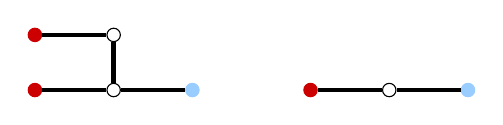
\begin{tikzpicture}
    \begin{scope}[yscale = 0.7, xscale = 0.5]
        \node[rvertex](r1) at (-2,0){};
        \node[rvertex](r2) at (-2,1){};
        \node[bvertex](b1) at (2,0) {};
        \node[evertex](v1) at  (0,0) {};
        \node[evertex](v2) at  (0,1){};

        \draw[tedge] (r1) -- (v1);
        \draw[tedge] (r2) -- (v2);
        \draw[tedge] (v1) -- (v2);
        \draw[tedge] (v1) -- (b1);
    \end{scope}

    \begin{scope}[yscale = 0.7, xscale = 0.5, shift = {(7,0)}]
        \node[rvertex](r1) at (-2,0){};
        \node[evertex](v1) at (0,0){};
        \node[bvertex](b1) at (2,0){};

        \draw[tedge] (r1) -- (v1);
        \draw[tedge] (v1) -- (b1);
        
    \end{scope}
\end{tikzpicture}
            \caption{A component of size $2$ (left) and a component of size $1$ (right).}\label{fig-t12}
        \end{figure}
       

        Recall that by Claim~\ref{C-Private}, every red vertex which is adjacent to a component~$K$ of $G[Z]$ of size~$2$ has exactly one uncoloured neighbour which is inside $K$.
        We say that a coloured vertex $v$ has property $Q$ if every uncoloured neighbour of $v$ has to be coloured with the same colour as $v$.
        



        \begin{myclaim}\label{c-p4p6-propertypropagates}
           Suppose that a coloured vertex $v$ satisfies $Q$, then we can colour the whole component of $H$ containing $v$ by propagation or conclude that $G$ has no red-blue colouring which extends the current partial colouring.
        \end{myclaim}
        \begin{claimproof}
        Let $v$ be a coloured vertex satisfying $Q$. Let $T$ be the set of uncoloured neighbours of $v$. Suppose that there is a vertex $w$ in $T$ with a second coloured neighbour $u$. By R2, $u$ has the opposite colour of $v$. Thus, if we colour $w$ according to $Q$, that is, with the colour of $v$, $u$ has a neighbour of the other colour and thus all other neighbours of $u$ have to have the same colour as $u$ and $Q$ is satisfied for $u$.

        Thus, if a vertex $v$ satisfies $Q$, then, after propagation, the coloured vertices at distance~$2$ of $v$ satisfy $Q$ and the uncoloured neighbours of $v$ are coloured. We continue the propagation exhaustively and either obtain a contradiction to the validity of the colouring and discard the branch, or the whole component is coloured.        
        \end{claimproof}


        \begin{myclaim}\label{C-Propagation}
        Let $T$ be a connected component of $G[Z]$ of size $2$. If we colour $T$ red and propagate the colouring, then either we obtain a valid red-blue colouring of~$H$ or we conclude that $T$ is be blue in any valid red-blue colouring of $H$.
        \end{myclaim}
        \begin{claimproof}
            Let $T$ be a connected component of $G[Z]$ of size $2$. We colour the vertices of $T$ red. Then, the neighbours of $T$ satisfy property $Q$. For the two red neighbours of $T$, this follows immediately from Claim~\ref{C-Private}. For the blue neighbour of $T$, this follows since $T$ gets coloured red.
            The claim follows from application of Claim~\ref{c-p4p6-propertypropagates}.
        \end{claimproof}

        \smallskip\noindent
        Let $k = \lvert \{ C | C \textrm{ is a connected component of size $2$ of $G[Z]$} \} \rvert$ be the number of connected components of size~$2$ in $G[Z]$. If $k=0$, we conclude by applying Lemma~\ref{L-Indep Set}.
        
        Otherwise, let $T\in H$ be a connected component of size $2$. 
        First, we colour $T$ red. By Claim~\ref{C-Propagation}, we either obtain in polynomial time a valid red-blue colouring and remember its value or we get that no such colouring exists and discard the branch.
        Second, we colour $T$ blue and propagate the resulting colouring. Then only $k-1$ components of size $2$ remain and we can repeat the same process and try to colour in red the uncoloured vertices of some component of size $2$.


    If at any point in our algorithm we discard a branch, we consider the next. For every valid red-blue colouring which we obtain, we remember its value and output the colouring with the minimum value. The correctness of our algorithm follows from its description. In the following, we analyse its run-time.

    By Lemma~\ref{l-propsafe}, the propagation of a colouring can be done in polynomial time. We consider $O(n^{48})$ branches, each of which can be processed in polynomial time. Therefore, the run-time of our algorithm is polynomial.
    \qed
\end{proof}




\begin{theorem}\label{t-p7}
    \minmc{} is polynomial-time solvable for $P_7$-free graphs.
\end{theorem}

\begin{proof}
    Let $G$ be a $P_7$-free graph. We assume that $G$ is connected. 
    We apply Observation~\ref{o-cutcolouring} and search for a minimum red-blue colouring of $G$. Theorem~\ref{T-Pk} states that $G$ has either a dominating $P_5$ or a dominating connected $P_5$-free subgraph and that such a subgraph can be found in polynomial time. If $G$ has a dominating $P_5$, we have a dominating set of bounded size and apply Lemma~\ref{l-smalldomset}. 
    In polynomial time, we either find a minimum red-blue colouring or conclude that no such colouring exists.

    Hence, we may assume that $G$ has a dominating set $D$ such that $G[D]$ is connected and $P_5$-free. By applying Theorem~\ref{T-Pk} again, we obtain that $G[D]$ either has a dominating $P_3$ or a connected dominating $P_3$-free subgraph.
    Note that a connected $P_3$-free subgraph is either a monochromatic clique, that is, a clique of size $1$ or at least $3$ or a clique of size $2$, that is, a $P_2$.
    We will distinguish between these two cases.
    


\smallskip
\noindent
\textbf{Case 1: }\textit{$G[D]$ is dominated by a monochromatic clique}\\ 
    Let $K$ be a clique of size $1$ or at least~$3$ in $G$ which dominates $G[D]$. Hence, every vertex of $G$ is at distance at most $2$ from $K$. Without loss of generality, we may colour $K$ red. 
    Consider first the case where all neighbours of $K$ are coloured red. Then, $N(K) \cup K$ dominates~$G$ and we apply Lemma~\ref{L-monodom}. We either obtain a valid red-blue colouring of $G$ and remember its value, or conclude that no such colouring exists and discard the branch.
    Otherwise, if $N(K) \cup K$ is not monochromatic, there is at least one blue vertex adjacent to $K$. We branch over all $O(n)$ options to colour a neighbour of $K$ blue and propagate the colouring using R1--R5. If we get a no-answer, we discard the branch, otherwise, we continue.
    Let $R$ (resp.~$B$) be the set of red (resp.~blue) vertices and let $Z$ be the set of uncoloured vertices. Observe that both $R$ and $B$ are connected in~$G$.

    If every connected component of $G[Z]$ is of size~$1$, we apply Lemma~\ref{L-Indep Set}. We either obtain a minimum red-blue $(R,B)$-colouring of $G$ and remember its value, or conclude that no such colouring exists and discard the branch.
    Therefore, we may assume that there is a connected component $C$ of $G[Z]$ of size at least~$2$.
    Recall that by R4, $C$ has to be adjacent to $B$. Let $x,y \in C$ such that $x$ and $y$ are adjacent and $x$ is adjacent to a blue vertex $b \in B$. Let $\beta$ be a blue neighbour of~$K$ which minimises $\dist_B(b,\beta)$. Let $b \, p_1 \, \dots \, p_\ell \, \beta $ be the shortest path in $B$ from $b$ to $\beta$.
    Note first that due to R3, not both of $x$ and $y$ may be adjacent to the same vertex in $p_1, \dots, p_\ell$. This allows us to assume that neither $x$ nor $y$ is adjacent to any of $p_1, \dots, p_\ell$, otherwise, if $p_j$, $j \in \{1,\dots, \ell\}$, is adjacent to $x$ or $y$, after potentially changing the role of $x$ and $y$, we replace $b$ by $p_j$.
    Let $\alpha \in K$ be the red neighbour of $\beta$.

    
    We claim that the path $y \, x \, b \,  p_{1} \dots  p_\ell \, \beta \, \alpha$ is induced.    
        Note first that $b \, p_1  \dots  p_\ell \, \beta$ is an induced path since it was chosen as a shortest blue path from $b$ to $\beta$. By construction, $x$ and $y$ are not adjacent to any of $p_1,\dots,p_\ell$ and $y$ is not adjacent to $b$. Since $\beta$ and $\alpha$ are neighbours of different colour, their other neighbours are coloured alike and neither $x$ nor $y$ can be adjacent to them. In addition, $\alpha$ cannot have a second blue neighbour in $\alpha, p_1, \dots, p_\ell$. Hence, the path is induced.
    Note that $\ell\leq 1$, since otherwise $y \, x \, b \,  p_{1}\, \dots \, p_\ell \, \beta \, \alpha$ is an induced $P_7$, a contradiction.



    

    \begin{myclaim} \label{c-p7-monoclique-yblue}
        If $y$ is coloured blue we can find in polynomial time a minimum red-blue $(R,B)$-colouring of $G$ or conclude that no such colouring exists.
    \end{myclaim}
    \begin{claimproof}
        We colour $y$ blue and propagate the colouring. Hence, by~R2, $x$ is blue as well. We branch over the $O(n^4)$ colourings of the neighbours of $b, x,y$ and $p_1$ (if it exists).

        Let $Q \subseteq R$ be the set of red neighbours of $b, x,y$ and $p_1$ (if it exists). Note that due to R2, $\lvert Q \rvert \leq 4$. Note that all neighbours of $Q$ except $b,x,y$ and $p_1$ are red by propagation. Let $S \subseteq R$ be the set of vertices of $R \setminus Q$ that are not in the same connected component as $\alpha$ in $G[R \setminus Q]$. 
        Note that $S$ might be empty.
        We partition $G[Z]$. Let $C_1 \subseteq Z$ be the set of uncoloured vertices with a red neighbour in $S$. Let $C_2 \subseteq Z$ be the set of uncoloured vertices with a red neighbour in $R\setminus (Q \cup S)$. Let $C_3$ be the set of uncoloured vertices without a red neighbour. Recall that the neighbours of $Q$ have already been coloured.

        Suppose for a contradiction that $C_2$ is not empty. Let $u \in C_2$ and let $u \, c_1 \, \dots \, c_k \, \alpha$ be the shortest path using vertices in $R\setminus (Q \cup S)$ from $u$ to $\alpha$. Since $u \in C_2$, such a path exists and since the neighbours of $\alpha$ are coloured, $k \geq 1$. Note further that the path is induced, since it is a shortest path.
        We claim that $P' = u \, c_1 \, \dots \, c_k \, \alpha \, \beta \, (p_1)\, b \, x \, y$ is an induced path of length at least $7$. 
        We already saw that $\alpha \, \beta \, (p_1)\, b \, x \, y$ is an induced path. By construction, $u \, c_1 \, \dots \, c_k \, \alpha$ is also an induced path. The red neighbours of $b$, $x$, $y$ and $p_1$ are in $Q$ and all their neighbours are coloured. Hence, they are not adjacent to any vertex of $c_1,\dots,c_k$ or $u$. Since the neighbourhood of $\beta$ is coloured blue except for $\alpha$, $\beta$ is neither adjacent to $u$ nor to any of $c_1, \dots, c_k$. Hence $P'$ is an induced path of length at least~$7$, a contradiction.
        It follows that $C_2$ is empty.

        Suppose for a contradiction that $C_3$ is not empty. Let $u \in C_3$ be an uncoloured vertex without a red neighbour. Since $u$ is at distance at most $2$ of $K$, there exist $w,z$ such that $z \in K$ and $w$ is adjacent to both $u$ and $z$. If $w$ is blue, $u$ would have been coloured by R2. Hence, $w$ is uncoloured and, as $z \notin S$, we get that $w \in C_2$. Since $C_2$ is empty, this is a contradiction. 
        It follows that $C_3$ is empty.
        
        Hence, $Z = C_1$ and is dominated by $R$.
        We apply Lemma~\ref{L-monodom} and either obtain a minimum red-blue $(R,B)$-colouring and remember its value or conclude that no such colouring exists and discard the branch.        
    \end{claimproof}
    


\noindent
We first check whether colouring $y$ blue leads to a valid red-blue $(R,B)$-colouring of $G$ in which case we remember its value. Note that this can be done in polynomial time by Claim~\ref{c-p7-monoclique-yblue}.
Then, we colour $y$ red and propagate the colouring. The number of uncoloured vertices decreased and we repeat the process from the point where we checked whether all connected components of $G[Z]$ have size~$1$.
Whenever we obtain a valid red-blue colouring, we remember its value. Whenever we discard a branch, we consider the next.
Initially, we consider $O(n)$ branches. In every iteration the number of uncoloured vertices decreases and we only recurse in the case where $y$ is red. Thus, we recurse at most $O(n)$ times and for each step in the recursion, we consider $O(n^4)$ sidebranches while considering the case where $y$ is blue, resulting in $O(n^{6})$ branches in total.
Since the application of Lemma~\ref{L-Indep Set} and the propagation can be done in polynomial time, our algorithm runs in polynomial time in the case where $G[D]$ is dominated by a monochromatic clique.

\smallskip
\noindent
    \textbf{Case 2: }\textit{$G[D]$ is dominated by a $P_2$ or a $P_3$}\\ 
    Let $P$ be a path in $G$ dominating $G[D]$ which is a $P_2$ or a $P_3$. Then, every vertex of $G$ is at distance at most $2$ of $P$. 
    Let $P = x_1 \, x_2$ if $D$ is dominated by a $P_2$ or else $P = x_1 \, x_2 \, x_3$. We branch over all colourings of~$P$. We denote by $R$ (resp.~$B$) the set of red (resp.~blue) vertices. If $P$ is monochromatic, we apply Lemma~\ref{l-ddmp} and either find a minimum red-blue $(R,B)$-colouring and remember its value or conclude that no such colouring exists and discard the branch.

	We now assume that $P$ is not monochromatic. By symmetry we may assume that $x_1$ is red and both $x_2$ and $x_3$ (if it exists) are blue. We branch over all $O(n^3)$ colourings of $N(P)$. Let $Z$ be the set of uncoloured vertices of $G$.
    If every vertex of $Z$ is adjacent to a blue vertex, then $B$ dominates $Z$ and we apply Lemma~\ref{L-monodom}. If we get a valid red-blue $(R,B)$-colouring of $G$, we remember its value, otherwise we get that no such colouring exists and discard the branch.
    
    Let $u\in Z$ be a vertex which is not adjacent to any vertex in $B$. As $u$ is at distance at most~$2$ of $P$ and the neighbourhood of $P$ is coloured, there is a vertex $r \in R$ which is adjacent to both $u$ and $x_1$. Let $C$ be the connected component of $u$ in $G[Z]$. Due to the application of R4, we know that $C$ is adjacent to $B$. Since $u$ is not adjacent to $B$, it has a neighbour $v \in C$, see Figure~\ref{f-p7-dom-p2}.

    \begin{figure}[t]
        \centering
        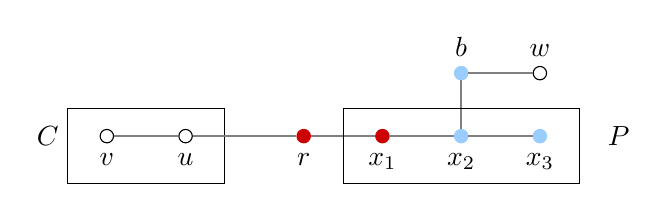
\begin{tikzpicture}
\begin{scope}
    \node[evertex, label=below:$v$](s2p) at (0,0){};
    \node[evertex, label=below:$u$](s1p) at (1,0){};

    %\node[bvertex, label = left:$b_2'$](b2p) at (-0.25, 1){};
    %\node[rvertex, label = right:$q_2'$](q2p) at (0.25,1){};
    %\node[rvertex, label = right:$q_1'$](q1p) at (1,1){};

    \draw[edge](s1p) -- (s2p);
    %\draw[edge](s1p) -- (q1p);
    %\draw[edge](s2p) -- (q2p);
    %\draw[edge](s2p) -- (b2p);

    \draw[] (-0.5, -0.6) rectangle (1.5,0.35);
    \node[] (c) at (-0.75,0){$C$};
    
\end{scope}


\begin{scope}[shift = {(2.5,0)}]
    \node[rvertex, label = {below:$r$}](t0) at (0,0){};
    \node[rvertex, label = below:$x_1$](t1) at (1,0){};
    \node[bvertex, label = below:$x_2$](tk1) at (2,0){};
    \node[bvertex, label = {below:$x_3$}](tk) at (3,0){};
    \node[bvertex, label = above:$b$](b) at (2,0.8){};
    \node[evertex, label = above:$w$](w) at (3,0.8){};

    \draw[edge](t0) -- (t1);
    \draw[edge](t1) -- (tk1);
    \draw[edge](tk1) -- (tk);
    \draw[edge](tk1) -- (b);
    \draw[edge](b) -- (w);

    \draw[] (0.5,-0.6) rectangle (3.5,0.35);
    \node[] (bw) at (4, 0){$P$};

    
    
\end{scope}



    \draw[edge](s1p) -- (t0);
    %\draw[edge](s1) -- (tk);

\end{tikzpicture}
        \caption{The path $P$ together with a component $C$ of size at least~$2$.}
        \label{f-p7-dom-p2}
    \end{figure}

    \begin{myclaim}\label{C-IndP6}
       $P' = v \, u \, r \, x_1 \, x_2 \, x_3$ is an induced path.
    \end{myclaim}

    \begin{claimproof}
        To see this, recall that $x_1 \, x_2 \, x_3$ is an induced $P_3$. 
        Since $u$ and $v$ are both uncoloured, they cannot be adjacent to $P$ and at most one can be adjacent to $r$.
        Further, if $r$ was adjacent to $x_2$ or $x_3$, $u$ would have been coloured red.
        Thus, $P'$ is an induced path.
    \end{claimproof}


    \begin{myclaim} 
    If $v$ is coloured red, we can find in polynomial time a minimum red-blue $(R,B)$-colouring of $G$ or conclude that no such colouring exists.
    \end{myclaim}
    \begin{claimproof}
    We colour $v$ red and propagate the colouring. Hence, by~R2, $u$ is red as well. We branch over the $O(n^3)$ colourings of the neighbours of $r,u$ and $v$.
    If $Z$ is dominated by $R$ we apply Lemma~\ref{L-monodom}. We either obtain a red-blue $(R,B)$-colouring and remember its value or conclude that no such colouring exists and discard the branch.
    
    Let $w\in G[Z]$ be not adjacent to $R$. As $w$ is at distance~$2$ of $P$, there is a vertex $b$ adjacent to both $P$ and $w$, see Figure~\ref{f-p7-dom-p2}. We know that $b\in B$, since $N(P)$ is coloured and $b$ is not red. Further, $b$ cannot be adjacent to any vertex in $R$, otherwise $w$ would have been coloured. If $b$ is adjacent to $x_2$, then $v \, u \, r \, x_1 \, x_2 \, b \, w$ is an induced $P_7$, a contradiction.
    Otherwise, $x_3$ exists and $b$ is adjacent to only $x_3$ in $P$, then $v \, u \, r \, x_1 \, x_2 \, x_3 \, b$ is an induced $P_7$, a contradiction.
    \end{claimproof}

    \smallskip \noindent
    We first check whether colouring $v$ red leads to a valid red-blue colouring, in which case we remember its value.
	Then, we colour $v$ blue and propagate the colouring.
    Now the number of uncoloured vertices decreased and we check again whether $B$ dominates $Z$ and otherwise find another connected component of $G[Z]$ of size at least~$2$, try to colour the vertex in the role of $v$ red and repeat the whole process.
    Whenever we discard a branch, we consider the next. Whenever we obtain a valid red-blue colouring, we remember its value. In every iteration, the number of uncoloured vertices decreases and we only recurse in the case where $v$ is blue. Thus, we recurse at most $O(n)$ times, and for each step in the recursion, we consider $O(n^3)$ sidebranches in the case where $v$ is red. Together with the initial branching to colour the neighbours of $P$, we consider in total $O(n^{7})$ branches.
    Since the application of Lemma~\ref{L-monodom} and the propagation can be done in polynomial time, our algorithm runs in polynomial time in the case where $G[D]$ is dominated by a $P_2$ or $P_3$.
    
    

\medskip \noindent
The correctness of our algorithm follows from its description. If we found a valid red-blue colouring, we output the smallest value of any valid red-blue colouring we obtained, otherwise we return that no such colouring exists. Since in both cases our algorithm runs in polynomial time, the total running time is polynomial.
        \qed
\end{proof}








\section{Hardness Results}
\label{sec:hardness}


For our hardness results, we reduce from \textsc{Vertex Cover}.
A \emph{vertex cover} is a set $S$ of vertices such that every edge is incident to a vertex of $S$. In the problem \textsc{Vertex Cover}, we are given an instance $(G,k)$ and ask whether $G$ has a vertex cover of size~$k$.
The problem \textsc{Vertex Cover} is well known to be \NP-complete, see e.g.~\cite{Ka72}.

\begin{theorem}\label{t-3p3}
\minmc{} is \NP-hard for $3P_3$-free graphs of radius~$2$ and diameter~$3$.
\end{theorem}
\begin{proof}
Let $(G,k)$ be an instance of \textsc{Vertex Cover}. We construct a graph $G'$ from $G$, consisting of vertex gadgets, edge gadgets, and cover gadgets (which will ensure that every edge of $G$ is covered) as follows.
For each vertex $v \in V(G)$ we construct a \emph{vertex gadget} consisting of two cliques $C_v$ and $C_v'$,  where $C_v$ is of size $|E(G)| + 2$ and $C_v'$ of size $\max(3,\degree(v) +1)$, and two vertices $u_v$ and $u_v'$. We pick a vertex $w$ in $C_v$ and $w'$ in $C_v'$ and add the edges $u_vw, wu_v', u_vw', w'u_v'$ to the gadget, see Figure~\ref{fig:3p3_constr}.
\begin{figure}[t]
    \centering
    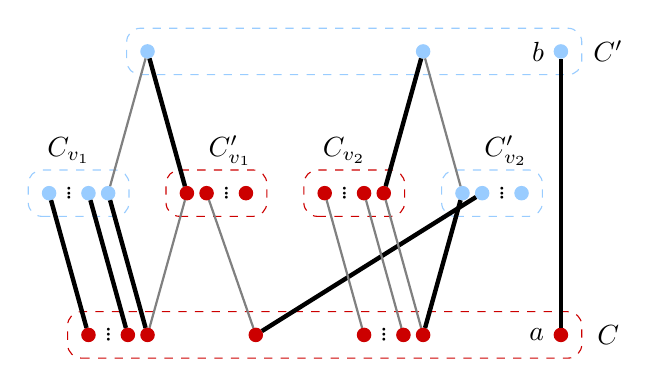
\begin{tikzpicture}
    \tikzset{
        rahmen/.style={
            rounded corners = 5pt,
            draw,
            dashed
        }
    }

    \newcommand{\vdotss}[2]{%
        \node at ($(#1)!0.5!(#2)$) {\hspace{0.7pt}\rotatebox{90}{$\cdot$\hspace{-1pt}$\cdot$\hspace{-1pt}$\cdot$}}%
    }
    \newcommand{\fframe}[3]{%
        \draw[rahmen,#1] ($(#2.north west)+(-0.4,0.4)$) rectangle ($(#3.south east)+(0.4,-0.4)$)%
    }
    \newcommand{\rclique}[2]{%
        \expandafter\node[vertex,draw=#1,fill=#1] (#2 k) at (0,1.5) {};
        \expandafter\node[vertex,draw=#1,fill=#1] (#2 2) at (0,0.5) {};
        \node[vertex,draw=#1,fill=#1] (#2 1) at (0,0) {};
        \vdotss{#2 2}{#2 k};
    }
    \newcommand{\clique}[2]{%
        \rclique{#1}{#2};
        \fframe{#1}{#2 k}{#2 1};
    }
    \newcommand{\iclique}[2]{%
        \expandafter\node[vertex,draw=#1,fill=#1] (#2 k) at (0,0) {};
        \expandafter\node[vertex,draw=#1,fill=#1] (#2 2) at (0,1) {};
        \node[vertex,draw=#1,fill=#1] (#2 1) at (0,1.5) {};
        \vdotss{#2 2}{#2 k};
        \fframe{#1}{#2 1}{#2 k};
    }

    \begin{scope}[xscale=0.5,yscale = 0.9, rotate = 90]
    %\begin{scope}[yscale=0.5]
    % v_1
    \rclique{nicered}{u};
    \begin{scope}[xshift=2cm,yshift=1cm]
        \clique{lightblue}{cu};
        \node[](t) at (0.6,1){$C_{v_1}$};
    \end{scope}
    \begin{scope}[xshift=2cm,yshift=-2.5cm]
        \iclique{nicered}{cpu};
        \node[](t) at (0.6,0.4){$C_{v_1}'$};
    \end{scope}
    \node[bvertex] (up) at (4,0) {};

    % v_2
    \begin{scope}[yshift=-7cm]
        \rclique{nicered}{v};
        \begin{scope}[xshift=2cm,yshift=1cm]
            \clique{nicered}{cv};
            \node[](t) at (0.6,1){$C_{v_2}$};
        \end{scope}
        \begin{scope}[xshift=2cm,yshift=-2.5cm]
            \iclique{lightblue}{cpv};
            \node[](t) at (0.6,0.4){$C_{v_2}'$};
        \end{scope}
        \node[bvertex] (vp) at (4,0) {};
    \end{scope}

    \node[rvertex] (e) at ($(u 1)!0.5!(v k)$) {};

    \node[rvertex, label = left:$a$] (a) at (0, -10.5) {};
    \node[bvertex, label = left: $b$] (b) at (4, -10.5) {};
    
    \fframe{nicered}{u k}{a};
    \node[](t) at (0,-11.7){$C$};
    \fframe{lightblue}{up}{b};
     \node[](t) at (4,-11.7){$C'$};
    
    \draw[tedge] (a) -- (b);

    % edge
    \draw[edge] (e) -- (cpu 2);
    \draw[tedge] (e) -- (cpv 2);

    % v_1
    \draw[tedge] (u 1) -- (cu 1);
    \draw[tedge] (u 2) -- (cu 2);
    \draw[tedge] (u k) -- (cu k);
    \draw[edge] (cu 1) -- (up);
    \draw[edge]  (u 1) -- (cpu 1);
    \draw[tedge] (cpu 1) -- (up);

    % v_2
    \draw[edge] (v 1) -- (cv 1);
    \draw[edge] (v 2) -- (cv 2);
    \draw[edge] (v k) -- (cv k);
    \draw[tedge] (cv 1) -- (vp);
    \draw[tedge]  (v 1) -- (cpv 1);
    \draw[edge] (cpv 1) -- (vp);
    \end{scope}

    %\end{scope}
\end{tikzpicture}
    \caption{
    The graph $G'$ constructed for a two adjacent vertices $v_1$ and $v_2$. 
    The given colouring indicates that $v_1$ is in the vertex cover $S$ while $v_2$ is not.
    }
    \label{fig:3p3_constr}
\end{figure}
We let $C$ and $C'$ be cliques with vertex sets $\{u_v, v \in V(G)\}$ and $\{u_v', v \in V(G)\}$, respectively. That is, we connect the vertices $u_v$ and $u_v'$ of the variable gadgets to two cliques $C$ and $C'$.

Consider an edge $e = vv'$ in $E(G)$.  We construct an \emph{edge gadget} as follows.
Pick a vertex $w \in C_{v}'$ and a vertex $w' \in C_{v'}'$, such that $w$ and $w'$ do not have a neighbour outside of $C_v'$ and $C_{v'}'$.
Add a new vertex $e$ to $C$ and add the edges $ew, ew'$.

For each $v \in V(G)$, we add $|E(G)| + 1$ vertices to $C$. We connect these vertices to $|E(G)|+1$ vertices in $C_v$ such that each of these vertices in $C_v$ has exactly one neighbour among the additional vertices in $C$ and vice versa. We call this the \emph{cover gadget} of $v$.

As a last step, we add vertices $a$ to $C$ and $b$ to $C'$ together with the edge $ab$.
Note that when adding vertices to $C, C'$ and $C_v$, for $v \in V(G)$, we add edges such that these sets remain cliques.

We first show that $G'$ is $3P_3$-free and has radius~$2$ and diameter~$3$.
To see that $G'$ is $3P_3$-free, note first that $G' - (C+C')$ is a disjoint union of cliques and thus contains no induced path consisting of more than $2$ vertices. Hence, every induced $P_3$ in $G'$ contains at least one vertex of one of the cliques $C$ and $C'$. Since no two induced paths can contain a vertex in the same clique, we conclude that $G'$ is $3P_3$-free.
The distance from $a$ to any vertex in $C$ and to $b$ is one. Since every vertex in the cliques $C_v$ and $C_v'$ for any $v \in V(G)$ is adjacent to a vertex in $C$, their distance to $a$ is two. Further, since the distance of any vertex in $C'$ to~$b$ is one, the distance to $a$ is two and thus $G'$ has radius~$2$.
The distance between any two vertices in $C$ and $C'$ is at most~$3$, which also holds for any two vertices in $G'- (C + C')$. Thus, the diameter of $G'$ is at most~$3$.

\medskip
\noindent
We claim that $G$ has a vertex cover of size $k$ if and only if $G'$ has a matching cut of size $\mu$ satisfying
\begin{equation}
\label{eq:p3free}
2|V(G)| + (1+|E(G)|)k + 1 \leq \mu \leq 2|V(G)| + (1 + |E(G)|)k + |E(G)| + 1
\end{equation}
Note that by Observation~\ref{o-cutcolouring} this is the case if and only if $G'$ has a red-blue colouring of value $\mu$.

First, suppose that $G$ has a vertex cover $S$ of size $k$. We construct a red-blue colouring as follows.
We colour $C$ red and $C'$ blue.
Let $v \in V(G)$. If $v \in S$ then colour $C_v$ blue and $C_v'$ red, otherwise colour $C_v$ red and $C_v'$ blue.
To see that this colouring is valid, note first that every vertex has at most two neighbours outside of the clique in which it is contained.
Let $v \in C$ be a vertex contained in a vertex gadget. Then, since $C_v$ and $C_v'$ are coloured differently, $v$ has at most one blue neighbour. By the same argument, a vertex $v' \in C'$ contained in a vertex gadget has at most one red neighbour.
Every vertex in $C_v$ and $C_v'$ has at most one neighbour in $C$ and one in $C'$, so regardless of its colour it has at most one neighbour of the other colour.
Consider a vertex $e \in C$, corresponding to an edge $e = uv$ of~$G$. Since $S$ is a vertex cover, at least one of $u$ and $v$ is contained in $S$ and thus at least one of $C_u'$ and $C_v'$ is red. 
All other vertices in $C$ or $C'$ have at most one neighbour outside of their clique. 

We compute the value of the colouring. Every vertex gadget has two bichromatic edges, so the vertex gadgets contribute a value of $2|V(G)|$.
Every edge gadget contains $0$ or $1$ bichromatic edge, thus their contribution is between $0$ and $|E(G)|$.
For the cover gadgets, if a vertex $v \in V(G)$ is contained in $S$, then the corresponding cover gadget contributes a value of $|E(G) + 1|$ and otherwise contributes a value of $0$.
Finally, the edge $ab$ contributes one to the value of the colouring.
In total, the value $\mu$ of the red-blue colouring satisfies Equation~(\ref{eq:p3free}).

\medskip \noindent
We now consider a fixed red-blue colouring of $G'$ of value $\mu$ satisfying Equation~(\ref{eq:p3free}) for some $k\in\mathbb N$.
Note first that the cliques $C$, $C'$, and $C_v$ and $C_v'$ for all $v \in V(G)$ are monochromatic in any valid red-blue colouring of $G'$.
\begin{myclaim}\label{c:3p3:cliquesdiffer1}
The cliques $C$ and $C'$ have different colours in every valid red-blue colouring of~$G'$.
\end{myclaim}
\begin{claimproof}
Suppose for a contradiction that they have the same colour, say $C$ and $C'$ are both red.
Then for every $v \in V(G)$ the vertices in $C_v$ and $C_v'$ that are adjacent to both $C$ and $C'$ have each two red neighbours and are thus red.
Hence, the cliques $C_v$ and $C_v'$ are all red, and thus all vertices of $G'$ are red, a contradiction.
\end{claimproof}

\begin{myclaim}\label{c:3p3:cliquesdiffer2}
For any $v \in V(G)$, the cliques $C_v$ and $C_v'$ have different colours in every valid red-blue colouring of $G'$.
\end{myclaim}
\begin{claimproof}
Suppose that both are coloured the same, say both are red. Then the blue vertex $v' \in C'$, which is adjacent to one vertex of each of $C_v$ and $C_v'$, has two red neighbours, a contradiction.
\end{claimproof}

\smallskip\noindent
Thus, each vertex gadget contributes a value of $2$ in every valid red-blue colouring of $G'$ .
Further, every edge gadget contributes a value of at most~$1$, since its vertex in $C$ has at most one neighbour of the other colour.
Also, the edge $ab$ is bichromatic and thus, contributes a value of $1$.

Without loss of generality and due to Claim~\ref{c:3p3:cliquesdiffer1} we may assume that $C$ is red and $C'$ is blue.
We define a set $S$ containing all vertices $v \in V(G)$ such that $C_v$ is coloured blue.

Note that a cover gadget for some $v \in V(G)$ contributes $(1 + |E(G)|)$ bichromatic edges if and only if the clique $C_v$ is blue, that is, if and only if $v \in S$.
From Equation~(\ref{eq:p3free}) we immediately get $(1 + |E(G)|)k \leq \mu - 2|V(G)| - 1 \leq (1 + |E(G)|)k + |E(G)|$ and thus there are 
$\left\lfloor \frac{\mu - 2|V(G)| - 1}{1 + |E(G)|} \right\rfloor = k$ vertices in $S$.

It remains to show that $S$ is a vertex cover of $G$.
Consider an edge $uv \in E(G)$. $S$ is a vertex cover if at least one of $u$ and $v$ is in $S$. 
That is, at least one of $C_u$ and $C_v$ has to be blue.
Suppose that this is not the case, that is, both $C_u$ and $C_v$ are red and thus, by Claim~\ref{c:3p3:cliquesdiffer2} both $C_u'$ and $C_v'$ are blue. Since they are contained in an edge gadget and thus have a common red neighbour in $C$, this contradicts the validity of the colouring.
\qed
\end{proof}

\noindent
%FINAL OR JOURNAL VERSION: Note, for a similar result we might use the trick of Moshi, however this leads to larger radius/diameter.
If we replace the cliques by complete bipartite graphs, we obtain a similar result for bipartite graphs. However, the radius and diameter increase by~$1$ and the construction is not $3P_3$-free.

\begin{theorem}\label{t-biprad3}
\minmc{} is \NP-hard for bipartite graphs of radius~$3$ and diameter~$4$.
\end{theorem}
\begin{proof}
    Let $(H,k)$ be an instance of \textsc{Vertex Cover}.
    Let $G$ be the graph constructed for this instance in the proof of Theorem~\ref{t-3p3}.
    We construct a bipartite graph $G'$ with partition classes $A$ and $B$ as follows. Replace every clique $C$ of size~$k$ by a complete bipartite graph $C'$ with partition classes each of size~$k$.
    We say that a vertex $u \in V(C)$ corresponds to two vertices in $V(C')$, $u_a \in A\cap V(C')$ and $u_b \in B\cap V(C')$.
    Let $u, v\in V(G)$ and let $u_a,u_b, v_a$ and $v_b$ be the corresponding vertices.
    If $uv \in E(G)$ we add the edges $u_av_b$ and $u_bv_a$.

    Thus, $G'$ is clearly bipartite since each edge connects a vertex in $A$ with a vertex in $B$.
    To see that $G'$ has radius~$3$ and diameter~$4$ note first that this is an increase of~$1$ compared to the radius and diameter of $G$.
    Consider a path in $G$ which is used to show that the distance between $u$ and $v$ in $G$ is bounded.
    Note that the distance between $u_a$ and one of $v_a$ and $v_b$ equals $\dist(u,v)$.
    Since $v_a$ and $v_b$ are adjacent, we get that $\dist(u_a,v_a) \leq \dist(u,v) +1$ and $ \dist(u_a,v_b) \leq \dist(u,v) +1$.
    By symmetry, the same holds for $u_b$ and thus, $G'$ has radius~$3$ and diameter~$4$.
    %journal version: add figure

    We claim that $H$ has a vertex cover of size $k$ if and only if $G'$ has a matching cut of size~$\mu' = 2\mu$ where
    \[
2|V(G)| + (1+|E(G)|)k + 1 \leq \mu \leq 2|V(G)| + (1 + |E(G)|)k + |E(G)| + 1
\]
as in the proof of Theorem~\ref{t-3p3}.
Note that by Observation~\ref{o-cutcolouring} this is the case if and only if $G'$ has a red-blue colouring of value~$\mu'$.

First, suppose that $H$ has a vertex cover $S$ of size $k$.
We construct a red-blue colouring of $G$ of value~$\mu$ using the arguments from Theorem~\ref{t-3p3}.
For every vertex $u\in V(G)$, we colour $u_a$ and $u_b$ in $V(G')$ with the same colour as~$u$.
This immediately leads to a valid red-blue colouring of $G'$ of value $2\mu = \mu'$ since every bichromatic edge $uv$ in $G$ connects two vertices $u$ and $v$ which do not belong to the same clique and each such edge corresponds to two edges $u_av_b$ and $u_bv_a$ in~$G'$.

Consider now a fixed red-blue colouring of $G'$ of value~$\mu'$.
Then, two vertices $u_a$, $u_b$ corresponding to the same vertex $u$ in $G$ are coloured the same since they are contained in a complete bipartite graph with partition classes of size at least~$3$.
Thus, the red-blue colouring of $G$ where a vertex $u$ has the same colour as $u_a$ in $G'$ is a red-blue colouring of $G$ of value~$\mu$.
Using the arguments from Theorem~\ref{t-3p3} we obtain a vertex cover $S$ of $H$ of size $k$. \qed
\end{proof}


\section{Conclusion}
\label{sec:conc}


Combining our results with results from~\cite{Ch84} and~\cite{FLPR23}, we obtain the following partial complexity classification for \minmc{} and we can update the classification for \mc.

\begin{theorem}[\cite{Ch84,FLPR23}]\label{t-h-dicho}
    For a graph $H$, \minmc{} on $H$-free graphs is \vspace{-7pt}
    \begin{itemize}
        \item polynomial-time solvable if $H \subseteq_i sP_2 + S_{1,1,2}$, $sP_2 + P_7$, or $sP_2 + P_6 + P_4$, for some $s \geq 0$, and
        \item \NP-hard if $H \supseteq_i 3P_3, K_{1,4}, C_r, r\geq 3$, or $H_i^*, i \geq 1$.
    \end{itemize}
\end{theorem}

\begin{theorem}[\cite{Ch84,FLPR23,LL23,LPR22,LPR23a,Mo89}]
For a graph $H$, \mc{} on $H$-free graphs is \vspace{-7pt}
\begin{itemize}
    \item polynomial-time solvable if $H \subseteq_i sP_3 + S_{1,1,2}$, $sP_3 + P_6 + P_4$ or $sP_3 + P_7$, for some $s \geq 0$, and
    \item NP-complete if $H \supseteq_i K_{1,4} , P_{14} , 2P_7 , 3P_5 , C_r$, $r \geq 3$, or $H_i^*$, $i \geq 1$.
\end{itemize} 
\end{theorem}

\noindent
In both cases, the computational complexity remains open only for a constant number of graphs $H$. In all open cases, every connected component of $H$ is either a path or a subdivided claw. This leads to the following natural open problem.

\smallskip\noindent
%\begin{open}
\textbf{Open Problem 1} 
    Complete the complexity dichotomies for \minmc{} and \mc{} on $H$-free graphs.
%\end{open}




\smallskip\noindent
Also, the computational complexity of graphs of bounded maximum degree has been investigated for different variants of \mc. While \maxmc{} is known to be \NP-hard for graphs of maximum degree~$3$~\cite{LPR23b}, every graph with at least~$7$ vertices and maximum degree~$3$ has a matching cut. This leads to our second open problem.

%\begin{open}
\smallskip\noindent
\textbf{Open Problem 2} 
Determine the complexity of \minmc{} on graphs of maximum degree~$3$.
%\end{open}









\medskip\noindent
\textbf{Acknowledgement}
The authors thank Van Bang Le for his valuable contributions to Theorem~\ref{t-s112}.
The authors further thank Clément Dallard, Daniel Paulusma, and Bernard Ries for fruitful discussions.
%
% ---- Bibliography ----
%
% BibTeX users should specify bibliography style 'splncs04'.
% References will then be sorted and formatted in the correct style.
%
 \bibliographystyle{splncs04}
 \bibliography{ref}





\end{document}
